% TODO: consistent references (the format of author names, years, pages, etc)

\documentclass[12pt,a4paper,english,twoside,openright]{report}
\usepackage{parskip}

\usepackage[includeheadfoot, inner=3.5cm, outer=3.5cm]{geometry}
\setlength{\headheight}{15pt}

\usepackage{emptypage}
\usepackage{pdfpages}

\usepackage{fancyhdr}
\pagestyle{fancy}
\fancyhf{}
\fancyhead[LE,RO]{\thepage}
\renewcommand{\sectionmark}[1]{ \markright{\thesection\ #1}{} }
\fancyhead[RE,LO]{\rightmark}

\usepackage{ragged2e}
\usepackage{adjustbox}
\usepackage{float}

\usepackage{multirow, array}
\usepackage{arydshln}

\usepackage[
  colorinlistoftodos,
  prependcaption,
  textsize=small
]{todonotes}

\usepackage[utf8]{inputenc}
\usepackage[T1]{fontenc,url}
\urlstyle{sf}

\usepackage[binary-units=true]{siunitx}
\DeclareSIUnit{\nothing}{\relax}
\newcommand{\kilo}[1]{\SI{#1}{\kilo\nothing}}
\newcommand{\mega}[1]{\SI{#1}{\mega\nothing}}
\newcommand{\micros}[1]{\SI{#1}{\micro\second}}
\newcommand{\millis}[1]{\SI{#1}{\milli\second}}
\newcommand{\seconds}[1]{\SI{#1}{\second}}
\newcommand{\mbytes}[1]{\SI{#1}{\mega\byte}}
\newcommand{\gbytes}[1]{\SI{#1}{\giga\byte}}

\usepackage{amssymb}
\usepackage{tikz}
\usetikzlibrary{matrix,arrows,backgrounds,fit}

\usepackage{forest}
\usepackage{pgfplots}
\usepgfplotslibrary{units}
\usepgfplotslibrary{groupplots}
\pgfplotsset{compat=1.16}

\usepackage{minted}
\newmintinline[ir]{rust}{}
\newmintedfile[rustfile]{rust}{}

\usepackage[noend]{algorithm,algpseudocode}
\makeatletter
\renewcommand{\ALG@beginalgorithmic}{\small}
\makeatother

\usepackage{babel,textcomp,csquotes,varioref,graphicx}

\usepackage[
  backend=biber,
  maxbibnames=6,
  isbn=false,
  doi=false,
  defernumbers=true
]{biblatex}
\addbibresource{refs.bib}
\setlength\bibitemsep{\baselineskip}

\usepackage[
  pdftitle={An RRB-tree based vector for Rust},
  pdfauthor={Araz Abishov},
  citecolor=linkblue,
  urlcolor=linkblue,
  colorlinks=true,
  linkcolor=black,
  unicode=true
]{hyperref}
\urlstyle{same}
\usepackage{cleveref}
\usepackage{xurl}

\raggedbottom

\newcommand{\dir}[1]{\mintinline[breaklines]{bash}{#1}}
\newcommand{\rust}[1]{\mintinline[breaklines]{rust}{#1}}
\newcommand{\type}[1]{\rust{#1}}
\newcommand{\crate}[1]{\emph{\textbf{#1}}}

\newcommand{\bigo}[1]{$\mathcal{O}(#1)$}
\newcommand{\bigochar}[1]{$\mathcal{O}$}
\newcommand{\range}[1]{#1}

\newcommand{\pvecrs}{\crate{pvec-rs}}
\newcommand{\imrs}{\crate{imrs}}
\newcommand{\rpds}{\crate{rpds}}
\newcommand{\rayon}{\crate{rayon}}

% Used to refer to the RRB-tree type
% provided by pvec-rs.
\newcommand{\rrbtree}{\type{RrbTree}}

% This macro is used to refer to the RRB-tree
% as a concept, rather than a concrete type
% provided by pvec-rs.
\newcommand{\treerrb}{RRB-tree}
\newcommand{\treerb}{RB-tree}

\newcommand{\refcell}{\type{RefCell}}
\newcommand{\boxptr}{\type{Box}}
\newcommand{\arc}{\type{Arc}}
\newcommand{\rc}{\type{Rc}}

\newcommand{\rbtree}{\type{RbTree}}
\newcommand{\rbvec}{\type{RbVec}}
\newcommand{\rrbvec}{\type{RrbVec}}
\newcommand{\pvec}{\type{PVec}}
\newcommand{\imrsvec}{\type{ImVec}}
\newcommand{\stdvec}{\type{Vec}}

\newcommand{\m}{$m$}
\newcommand{\h}{$h$}
\newcommand{\x}{$x$}
\newcommand{\nil}{\emph{NIL}}
\newcommand{\la}{$\leftarrow$}
\newcommand{\ts}[1]{\textsubscript{#1}}
\newcommand{\n}{\emph{N}}

\algnewcommand\And{\textbf{and}}
\algnewcommand\In{\textbf{in}}

\definecolor{linkblue}{HTML}{008CFF}
\definecolor{morange}{HTML}{FF9800}
\definecolor{mpurple}{HTML}{512DA8}
\definecolor{mred}{HTML}{D32F2F}
\definecolor{mgreen}{HTML}{689F38}

\title{A Vector Implementation Based On RRB-Tree for Rust}
\author{Araz Abishov}

\begin{document}

\pagenumbering{roman}
\includepdf[pages={-}]{forside/forside.pdf}
\setcounter{page}{5}

\pdfbookmark[0]{Front matter}{bm-frontmatter}
\pdfbookmark[1]{Contents}{bm-toc}
\tableofcontents{}

\cleardoublepage
\vspace*{2cm}
\thispagestyle{plain}

\phantomsection
\addcontentsline{toc}{section}{Abstract}

\begin{center}
\section*{Abstract}
\end{center}

Rust is a multi-paradigm system programming language focused on performance and reliability. Its rich type system guarantees memory and thread-safety at compile-time.

Rust forbids simultaneous sharing and mutation, that sometimes is a necessary and a useful pattern. A common way to mitigate this limitation in Rust is to clone a value before sharing it. Naive cloning by copying, however, is an expensive operation both in terms of memory and performance.

This thesis presents \pvecrs{}, a project that contributes a vector implementation with efficient clone operation that borrows ideas from persistent data structures. The project explores novel approaches to optimize vector’s performance by leveraging type system of Rust, as well as aiming to achieve convenient, idiomatic interface familiar to developers. The proposed optimizations are evaluated and discussed based on results of the sequential and parallel tests.


\cleardoublepage
\vspace*{2cm}
\thispagestyle{plain}

\begin{center}

\phantomsection
\addcontentsline{toc}{section}{Acknowledgements}

\section*{Acknowledgements}

\end{center}

I would like to thank my supervisors, Martin Steffen and Volker Stolz, for their guidance and feedback. Without their patience and support, as well as trust in my own idea, this venture would not have been possible.

My deepest appreciation goes to my family and my friends for their moral support, their continuous encouragement, and their help whenever it was needed.

Finally, I would like to thank the Rust community for being so welcoming and supportive. In particular, I am grateful to Nicholas D. Matsakis for inspiring me to work on this project.


\cleardoublepage
\thispagestyle{plain}

\begin{center}
    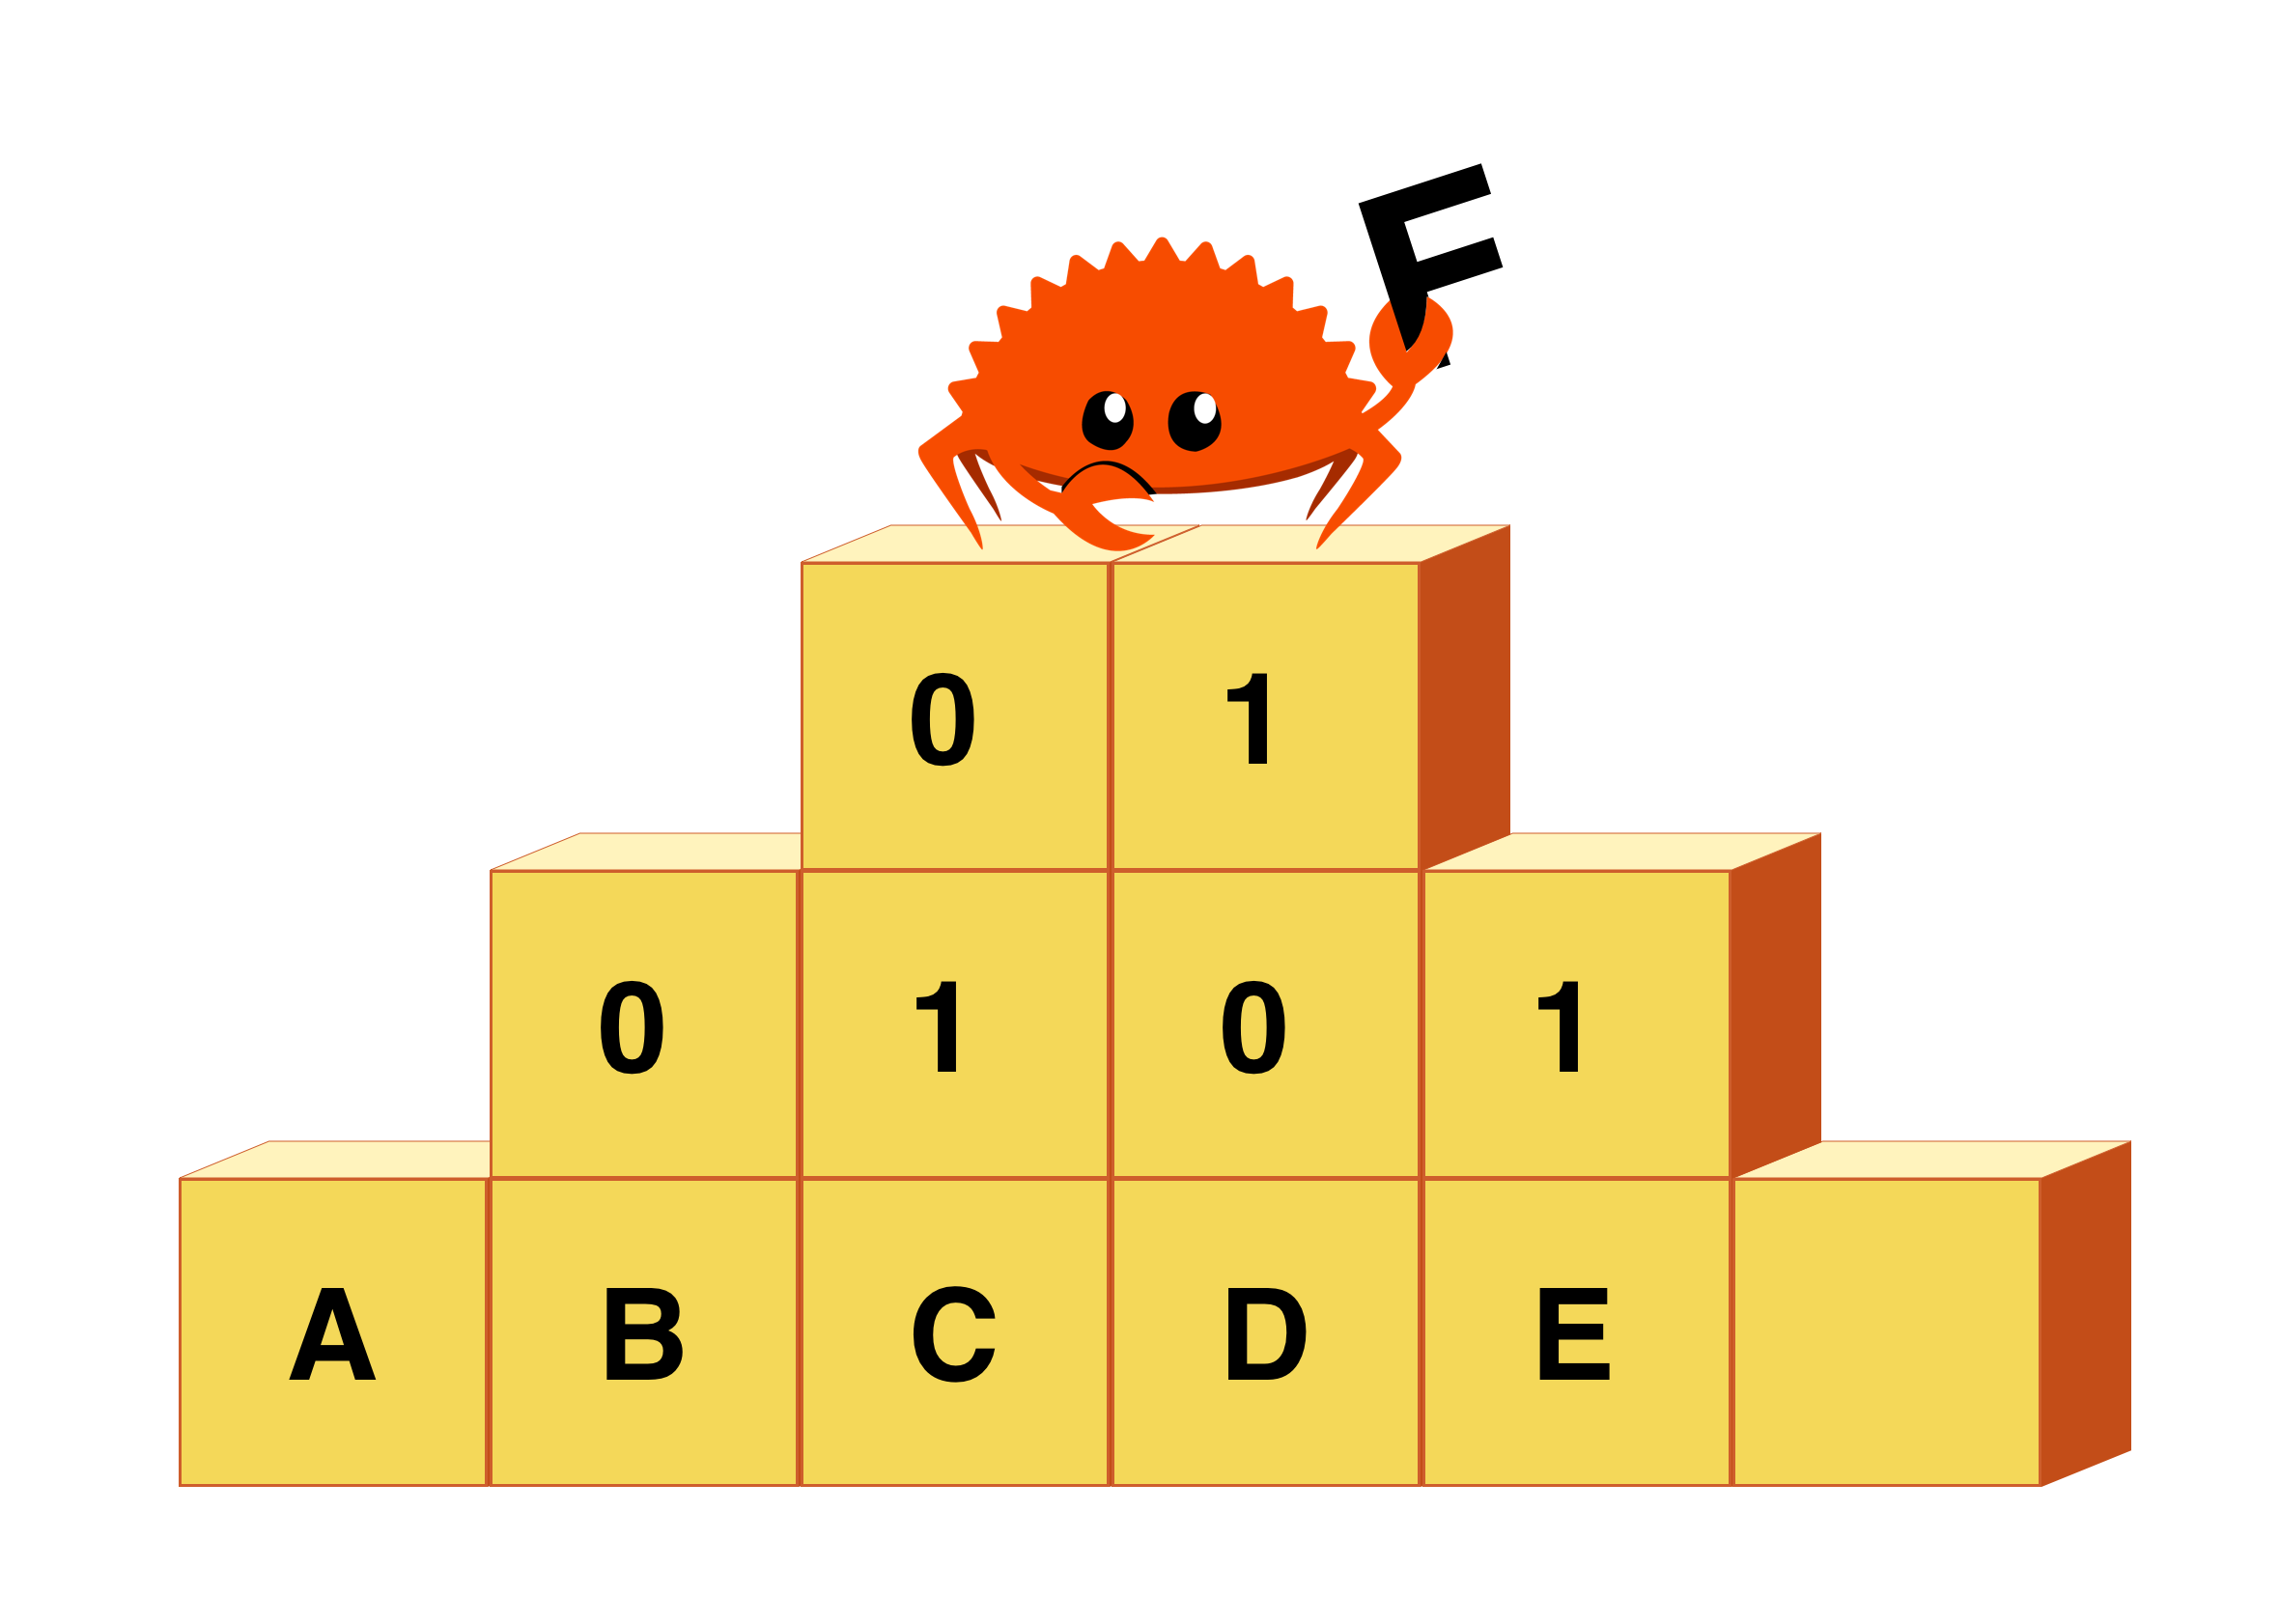
\includegraphics[width=8cm, angle=0, trim=10 10 10 10, clip]{images/ferris-climbing.png}

    \phantomsection
    \addcontentsline{toc}{section}{Reading notes}

    \section*{Reading notes}
    \begin{justify}
        The links to the LaTeX source code and the latest version of this document can be found at \url{https://abishov.com/thesis/}. The implementation, documentation, and visualization demo can be found at \url{https://abishov.com/pvec-rs}.

        If you notice any typos while reading the document, or have any feedback in general, feel free to open an issue at \url{https://github.com/arazabishov/thesis/issues} or send me an email at \href{mailto:araz@abishov.com}{\nolinkurl{araz@abishov.com}}.

        \paragraph{Colophon}
        The illustration above with Ferris\footnote{Unofficial mascot for Rust: \url{https://rustacean.net/}} sitting on top of \treerrb{}, kindly prepared by Vanessa Tesorone. The reading notes design and the idea to use Rust's mascot for the document decoration was inspired by the master's thesis of Erik Vesteraas\footnote{\url{http://erik.vestera.as/thesis/}}.
    \end{justify}

    \subsection*{Typographic conventions}
    \begin{tabular}{ r l }
        Clickable link & \href{https://www.rust-lang.org/}{Rust Programming Language} \\
        Inline code and types & \mintinline{rust}{Vec::new()} \\
        Project or library name & \pvecrs{} \\
    \end{tabular}

\end{center}


\cleardoublepage

\pagenumbering{arabic}
\chapter{Introduction}

% TODO: Optional<Add a point to introduction to describe what is RefCell>
% TODO: Linear types (from Jean's work):
% Earlier work has lead to the definition of linear types, a way to define mutable types in a similar fashion as transients, with focus on correctness [20]. A linear type can only be used once, although relaxed constraints provide means to temporarily define a linear type as nonlinear, which gives users read capabilities without “using” the instance. In contrast, a transient is an affine type, where the function persistent! converts the affine nodes permanently to nonlinear, persistent nodes. 
% TODO: Linear types can change the world

\section{Persistent data structures}

A vast majority of modern programming languages are equipped with a standard library --- a set of constructs and utilities aimed to improve the developer's productivity. 

A significant part of standard library consists of commonly used data structures such as lists, sets, and maps, which often provide operations for reading and writing data. 

Modifying or \emph{mutating} an \emph{ephemeral} data structure implies that we no longer will have access to its older version. In contrast, a \emph{persistent} data structure allows access to any version, old or new, at any time \cite{making-data-structures-persistent}. 

Persistent data structures could be classified based on the operations which they offer over their versions:
\begin{itemize}
    \item \textit{Partial persistence} --- In this persistence model, we can query any previous version of the data structure, but we can update only the newest version. The versions are linearly ordered. 
    \item \textit{Full persistence} --- Both access and updates are allowed on all versions. The versions can be visualized as a branching tree.
    \item \textit{Confluent persistence} --- In addition to the previous operations, it offers combination operation to merge more than one previous version to output a new single version. The versions form a directed acyclic graph \cite{fully-persistent-lists-with-catenation}.  
    \item \textit{Functional persistence} --- This model takes its name from functional programming where objects are immutable. In comparison to the previous models, it prohibits change of the internal representation of the data structure \cite{purely-functional-data-structures}. 
\end{itemize}

While persistence can be achieved by simple copying, the performance of a modification operation quickly becomes unacceptable. This led to research and development of more efficient solutions, which were often designed to solve particular problems. A lack of general purpose collections, which guarantee uniformly good performance across different operations, results in challenges with software development. 

A persistent \emph{vector}, also known as a one-dimensional growable array, is very inefficient if implemented naively. Each update operation will cause a full copy of the underlying array, consuming additional amount of memory and processor time. 

However most operations modify only some parts of data structures, a complete copy is redundant. A better approach is to exploit the similarity between the new and old versions by \emph{sharing} structure between them. For example, instead of representing a data structure as a single block of memory, it could be broken down into smaller pieces or \emph{nodes}, which are linked together in the form of a \emph{tree}. Since modifications only apply to some nodes, the rest of them still remain unchanged and can be shared without copying. 

The first persistent vector implementation which offered good performance across a broad range of operations was introduced by Rich Hickey in the Clojure programming language. It was based on Phil Bagwell's Hash Array Mapped Trie \cite{ideal-hash-trees}, which offers practically constant runtime for push, update, and access operations, and it is a \emph{fully} persistent data structure. 

Later Phill Bagwell introduced a confluently persistent vector based on Relaxed Radix Balanced Tree \cite{efficient-immutable-vectors}, which has improved performance of the concatenation operation significantly and became a foundation for Scala's standard library vector implementation. 

The project presented in the thesis contributes an efficient persistent vector implementation for Rust based on Relaxed Radix Balanced Tree, which takes advantage of the Rust's type system to improve performance, guarantee thread safety and provide an idiomatic application programming interface. In order to ensure the best possible average performance, its internal representation switches from standard vector to RRB-Tree during runtime. 

\section{The Rust programming language}
\todo{The Rust programming language}

\subsection{Ownership and borrowing}
\todo{Ownership and borrowing}

\subsection{Reference counting and memory management}
\todo{Reference counting and memory management}

\section{Contributions}
\todo{Contributions}

\chapter{Background}

This chapter gives an introduction to the \treerb{} and \treerrb{} data structures that are used as the foundation for persistent vectors:

\begin{itemize}
    \item First, we will take a look at \emph{radix balanced tree}, its organization, and algorithms such as \emph{radix search} and \emph{path copying} that are used at the core of all vector operations.
    \item Then, we will proceed to its extension --- \emph{relaxed radix balanced tree} that enables efficient concatenation and splitting.
    \item Finally, we will get an overview of what is \emph{transience} and how it can be used to improve the performance of persistent data structures.
\end{itemize}

\section{Radix balanced tree}
\label{chapter:radix-balanced-tree}

Radix balanced tree or \treerb{} is an \m{}-ary tree that uses integers as keys to find values. The data structure was pioneered by Rich Hickey as the foundation for the persistent vector implementation in Clojure \cite{the-clojure-programming-language}.

\treerb{} consists of nodes which reference other subtrees or values. We will be referring to the former and latter types of nodes as \emph{branches} and \emph{leaves} correspondingly. The number of subtrees and values in the node is configurable and will be defined as \m{} or the \emph{branching factor}. The branching factor can be any number that is a power of 2, allowing an efficient radix search implementation.

The higher the value of \m{} is, the wider and shallower the tree will be. From now on the height of a tree will be referred to as \h{}, where $h_{max}$ is the upper boundary:

\begin{equation}
    \label{eq:h-max}
    h_{max} = log_m(n)
\end{equation}

When \m{} is a large value, for example, 32, the tree becomes shallow, and the complexity of accessing values by traversing the tree from the root to a leaf becomes \emph{effectively} constant. For example, if the maximum value of 32 bit signed integer is substituted for $n$ in \Cref{eq:h-max} then $h_{max}$ will never exceed 7 levels. Thus, due to its strong performance guarantees, \treerb{} serves as a solid foundation for a general-purpose persistent vector implementation.

In the following sections, we will take a look at \treerb{} algorithms used to implement vector operations\footnote{For a formal definition of \treerb{}, refer to \cite{improving-performance-through-transience}}.

\subsection{Radix search}
\label{sec:rb-tree-radix-search}

An algorithm that is used to lookup values in \treerb{} is called \emph{radix search}. It serves as foundation for other operations that involve the tree traversal, such as push, pop, and update.

\subsubsection*{Bit partitioning}
Radix search accepts a key of the integer type as an argument. It can be thought of as a composite key, where each subkey is a sequence of bits. Conceptually, the idea is to divide the key into bit blocks, where each block is an index specific to the tree level.

As demonstrated in \Cref{eq:bits-per-level}, the bit block size can be calculated from the branching factor. It will be referred to as \x{} or \emph{bits per level}. When the branching factor \m{} is 16 \x{} is 4, meaning that the subkey size is equal to 4 bits.

\begin{equation}
    \label{eq:bits-per-level}
    x = log_2(m)
\end{equation}

\subsubsection*{Extracting subkeys}
The number of subkeys within the search key depends on the number of tree levels or \h{}. For example, a search key addressing an element of the tree of ${h = 3}$ and ${x = 2}$ will consist of 3 subkeys taking up 6 bits of space in total.

Subkeys are arranged in the order from the most to the least significant bits, where the most significant block of bits is a key used to access the child node of the root. Each following key is used to find a child node on the corresponding tree level.

Let us consider an example of processing a key that addresses a value in the tree of $h = 3$, $m = 4$ and $x = 2$.

\begin{equation}
    54_{10} = 00110110_2
\end{equation}

Since the tree height is three, we have three corresponding subkeys: $11_2$, $01_2$, and $10_2$. Let us assume that we are interested in extracting the subkey for the child node on the second level--$01_2$.

The first step is to get rid of the bits following the subkey of our interest. Logical right shift operation\footnote{A logical right shift is a bitwise operation that shifts all the bits of its first operand to the right by number of bits specified in the second operand.} denoted as $\ggg$, will push specified count of 0s into key $k$, where $l$ is the \emph{level} at which current node is located:

\begin{equation}
    k \ggg ((l - 1) \cdot x).
\end{equation}

Since the node from the example is located at $l = 2$ in the tree of $x = 2$, the key $k$ is shifted by 2 bits. The result of the operation is $00001101_2$. As a result, the "tail" of the key is truncated. The next step is to remove bits preceding the subkey by masking them to 0 using the bitwise "and" operator.

A bitwise "and" takes two equal-length binary representations and executes the "and" operation for each pair of the corresponding bits. If both bits in the compared position are 1, the bit in the resulting binary representation is 1; otherwise, the result is 0. Here is an example, where the first and the second operands are the key and mask respectively:

\begin{equation}
    00001101 \ \& \ 00000011 = 00000001.
\end{equation}

Only the last two bits of the mask are set to 1, meaning that all bits of the key except the last two will be masked to 0. The result of the "and"-ing operation will be the value of the subkey.

A mask must be of the same type as a key and can be calculated from the branching factor \m{}:

\begin{equation}
    \mathit{mask} = m - 1.
\end{equation}

If \m{} is equal to 4, the maximum subkey value will be 3, which equals to 00000011\ts{2}.

\begin{figure}[!ht]
    \colorlet{color-path}{blue!30}
    \colorlet{color-node}{blue!10}

    \centering
    \footnotesize
    \begin{tikzpicture} [
        node/.style={
            matrix of nodes,
            nodes={draw,minimum width=5mm,minimum height=6mm,anchor=center},
            inner sep=0pt,
            font=\ttfamily,
            nodes in empty cells
        },
        value/.style={
            matrix of nodes,
            nodes={draw=none,minimum width=5mm,minimum height=6mm,anchor=center},
            inner sep=0pt,
            font=\ttfamily,
            text height=1.5ex,
            text width=2.25ex,
            text centered,
            nodes in empty cells
        },
        edge/.style={->, shorten >= 4pt},
    ]
        \node[] (index) at (current page.north) { $104_{10}$ = $01 10 10 00_{2}$ };

        \matrix[node] (node-1-1) [below right=8mm and 1cm of index] { 00 & 01 & 10 & 11 \\ };

        \scoped[on background layer] {
            \node[fit=(node-1-1-1-1), fill=color-node, inner sep=0pt] {};
            \node[fit=(node-1-1-1-2), fill=color-path, inner sep=0pt] {};
            \node[fit=(node-1-1-1-3), fill=color-node, inner sep=0pt] {};
            \node[fit=(node-1-1-1-4), fill=color-node, inner sep=0pt] {};
        }

        \matrix[node, inner sep=0pt] (node-2-2) [below left=8mm and 1mm of node-1-1.south] { 00 & 01 & 10 & 11 \\ };
        \matrix[node, fill=color-node] (node-2-3) [below right=8mm and 1mm of node-1-1.south] { & & & \\ };
        \matrix[node, fill=color-node] (node-2-1) [left=2mm of node-2-2.west] { & & & \\ };
        \matrix[node, fill=color-node] (node-2-4) [right=2mm of node-2-3.east] { & & & \\ };

        \scoped[on background layer] {
            \node[fit=(node-2-2-1-1), fill=color-node, inner sep=0pt] {};
            \node[fit=(node-2-2-1-2), fill=color-node, inner sep=0pt] {};
            \node[fit=(node-2-2-1-3), fill=color-path, inner sep=0pt] {};
            \node[fit=(node-2-2-1-4), fill=color-node, inner sep=0pt] {};
        }

        \draw[edge, out=225, in=45] (node-1-1-1-1.south) to (node-2-1.north);
        \draw[edge, out=225, in=45] (node-1-1-1-2.south) to (node-2-2.north);
        \draw[edge, out=315, in=135] (node-1-1-1-3.south) to (node-2-3.north);
        \draw[edge, out=315, in=135] (node-1-1-1-4.south) to (node-2-4.north);

        \matrix[node, fill=color-node] (node-3-2) [below left=8mm and 1mm of node-2-2.south] { & & & \\ };
        \matrix[node, inner sep=0pt] (node-3-3) [below right=8mm and 1mm of node-2-2.south] { 00 & 01 & 10 & 11 \\ };
        \matrix[node, fill=color-node] (node-3-1) [left=2mm of node-3-2.west] { & & & \\ };
        \matrix[node, fill=color-node] (node-3-4) [right=2mm of node-3-3.east] { & & & \\ };

        \scoped[on background layer] {
            \node[fit=(node-3-3-1-1), fill=color-node, inner sep=0pt] {};
            \node[fit=(node-3-3-1-2), fill=color-node, inner sep=0pt] {};
            \node[fit=(node-3-3-1-3), fill=color-node, inner sep=0pt] {};
            \node[fit=(node-3-3-1-4), fill=color-path, inner sep=0pt] {};
        }

        \draw[edge, out=225, in=45] (node-2-2-1-1.south) to (node-3-1.north);
        \draw[edge, out=225, in=45] (node-2-2-1-2.south) to (node-3-2.north);
        \draw[edge, out=315, in=135] (node-2-2-1-3.south) to (node-3-3.north);
        \draw[edge, out=315, in=135] (node-2-2-1-4.south) to (node-3-4.north);

        \matrix[node, fill=color-node] (node-4-2) [below left=8mm and 1mm of node-3-3.south] { & & & \\ };
        \matrix[node, fill=color-node] (node-4-3) [below right=8mm and 1mm of node-3-3.south] { & & & \\ };
        \matrix[node, fill=color-node] (node-4-1) [left=2mm of node-4-2.west] { & & & \\ };
        \matrix[node, inner sep=0pt] (node-4-4) [right=2mm of node-4-3.east] { 00 & 01 & 10 & 11 \\ };

        \scoped[on background layer] {
            \node[fit=(node-4-4-1-1), fill=color-path, inner sep=0pt] {};
            \node[fit=(node-4-4-1-2), fill=color-node, inner sep=0pt] {};
            \node[fit=(node-4-4-1-3), fill=color-node, inner sep=0pt] {};
            \node[fit=(node-4-4-1-4), fill=color-node, inner sep=0pt] {};
        }

        \draw[edge, out=225, in=45] (node-3-3-1-1.south) to (node-4-1.north);
        \draw[edge, out=225, in=45] (node-3-3-1-2.south) to (node-4-2.north);
        \draw[edge, out=315, in=135] (node-3-3-1-3.south) to (node-4-3.north);
        \draw[edge, out=315, in=135] (node-3-3-1-4.south) to (node-4-4.north);

        \matrix[value] (node-5-1) [below = 0mm of node-4-1.south] { a & b & c & d \\ };
        \matrix[value] (node-5-2) [below = 0mm of node-4-2.south] { e & f & g & h \\ };
        \matrix[value] (node-5-3) [below = 0mm of node-4-3.south] { i & j & k & l \\ };
        \matrix[value] (node-5-4) [below = 0mm of node-4-4.south] { m & n & o & p \\ };
    \end{tikzpicture}

    \caption{Visualization of the radix search algorithm}
    \label{fig:rb-tree-example-1}
\end{figure}

\Cref{fig:rb-tree-example-1} is an illustration of how radix search works. There is only a fraction of the tree visualized in the example rendering values in the [92, 107] index range.

The branching factor of the tree is 4, resulting in the subkey size of 2 bits. The mask is equal to 3 or 00000011 in binary representation. For simplicity, the index type is selected to be \emph{unsigned byte} with a maximum capacity of 256.

The tree height in \Cref{fig:rb-tree-example-1} is 4. The goal is to lookup the value at the index 104, which is equal to 01101000\ts{2}. \Cref{lst:rb-tree-radix-search} outlines the radix search algorithm.

The search starts by initializing the node and level variables to root and $height - 1$ correspondingly. The for loop runs until the leaf node level is reached, where each step towards it involves selecting a child node by using bit shifting and masking. After exiting the loop, the function returns the value from the leaf node. The runtime complexity of radix search is \bigo{log_m(n)}.

\begin{listing}[ht!]

    \begin{algorithmic}[1]
        \Function{RadixSearch}{root, key}
            \State node \la\ root

            \For{level \la\ root\ts{height} - 1, 1}
                \State index \la\ (key $\ggg$ (level $\cdot$ x)) \& mask
                \State node \la\ node[index]
            \EndFor

            \State index \la\ key \& mask
            \State \Return {node[index]}
        \EndFunction
    \end{algorithmic}

    \caption{Radix search algorithm}
    \label{lst:rb-tree-radix-search}
\end{listing}

\subsection{Update}
The persistent \emph{update} operation returns a new tree version that includes an updated value, instead of mutating the original instance in-place as with \emph{ephemeral} data structures.

\subsubsection*{Path copying}
When updating a \treerb{}, the radix search algorithm is used to build a path to the value. In order to avoid mutating the original tree instance, each node on the path is copied. This process is called as \emph{path copying} \cite{planar-point-location}. It is important to emphasize that nodes that are not a part of the path are reused.

The update operation performs the \h{} count copies of \m{} sized nodes, where \h{} is the maximum height of the tree. As described in \Cref{eq:h-max}, \h{} is bound by \bigo{log_m(n)}, which results in {\bigo{m \cdot log_m(n)}} complexity of the update operation.

For large branching factors \m{} such as 32, the performance becomes effectively \bigo{1}. For example, if the tree is full, where the count of all elements $n$ is bound by the maximum value of 32 bit integer\footnote{2147483647}, \h{} will be at most 7.

\begin{listing}[ht!]
    \begin{algorithmic}[1]
        \Function{Update}{root, key, value}
            \State newRoot \la\ \Call{Clone}{root}
            \State node \la\ newRoot

            \For{level \la\ root\ts{h} - 1, 1}
                \State index \la\ (key $\ggg$ (level $\cdot$ x)) \& mask
                \State newChildNode \la\ \Call{Clone}{node[index]}
                \State node[index] \la\ newChildNode
                \State node \la\ newChildNode
            \EndFor

            \State index \la\ key \& mask
            \State node[index] \la\ value
            \State \Return newRoot
        \EndFunction
    \end{algorithmic}

    \caption{Path copying algorithm for \treerb{}}
    \label{lst:rb-tree-update}
\end{listing}

From the implementation perspective, the difference between update and radix search is that every visited node, including root, must be copied. The return value is the root node for the new version of the tree.

\subsection{Push}
The push operation is used to add new values to the end of \treerb{}. It employs \emph{path copying} to preserve the original tree without changes. It accepts the root node and new value as arguments and returns a new version of the tree.

The \treerb{} size is used as the search key. For example, if the tree size is 9, a key for the new value will be 9. The size is incremented after the operation completes.

Since the push operation adds new values, it has to manage the tree capacity. Generally, there are two cases that require special handling:

\begin{itemize}
    \item The case when a path to a leaf node includes branches that are not created yet. The solution is to generate missing nodes while descending the tree.
    \item The \emph{root overflow} or when the tree size exceeds its \emph{capacity}\footnote{Capacity is the maximum number of elements a tree can accommodate.}. It can be solved by adding a new level to the tree by creating a new root node and setting the old one as the first child of the new root.
\end{itemize}

The complexity of the operation is \bigo{m \cdot log_m(n)} as it traverses and creates new nodes from the root to a leaf.

\Cref{lst:rb-tree-push} demonstrates how the tree capacity is calculated and managed.

\begin{listing}[ht!]
    \begin{algorithmic}[1]
        \Function{Capacity}{height}
		    \State \Return m $\ll$ ((height - 1) $\cdot$ x)
        \EndFunction

        \State

        \Function{Push}{root, value}
            \State newRoot \la\ \nil{}

            \If{\Call{Capacity}{root\ts{height}} <= root\ts{size}}
                \State newRoot \la\ \Call{CreateNode}{}
                \State newRoot[0] \la\ \Call{Clone}{root}
                \State newRoot\ts{height} \la\ root\ts{height} + 1
            \Else
                \State newRoot \la\ \Call{Clone}{root}
            \EndIf

            \State node \la\ newRoot
            \State key \la\ newRoot\ts{size}

            \For{level \la\ newRoot\ts{height} - 1, 1}
                \State index \la\ (key $\ggg$ (level $\cdot$ x)) \& mask

                \State childNode \la\ node[index]
                \State newChildNode \la\ \nil{}

                \If{childNode = \nil{}}
                    \State newChildNode \la\ \Call{CreateNode}{}
                \Else
                    \State newChildNode \la\ \Call{Clone}{childNode}
                \EndIf

                \State node[index] \la\ newChildNode
                \State node \la\ newChildNode
            \EndFor

            \State index \la\ key \& mask
            \State node[index] \la\ value

            \State newRoot\ts{size} \la\ newRoot\ts{size} + 1
            \State \Return newRoot
        \EndFunction
    \end{algorithmic}

    \caption{Pseudocode for the \treerb{}'s push operation}
    \label{lst:rb-tree-push}
\end{listing}

\subsection{Pop}
The purpose of pop is to remove values from the end of \treerb{}. It accepts root as input and returns both a removed value and a new version of a structure.

Pop is responsible for reducing the capacity of \treerb{} when needed, including the removal of empty branches and leaves. Similar to update and push operations, it relies on the path copying algorithm to avoid modifying the existing version of the tree.

\begin{listing}[ht!]

    \begin{algorithmic}[1]
        \Function{PopNode}{node, key}
            \State newNode \la\ \Call{Clone}{node}
            \State value \la\ \nil{}

            \If{node\ts{height} = 0}
                \State index \la\ key \& mask
                \State value \la\ newNode[index]
                \State newNode[index] \la\ \nil{}
            \Else
                \State index \la\ (key $\ggg$ (newNode\ts{height} $\cdot$ x)) \& mask
                \State value, childNode \la\ \Call{PopNode}{newNode[index], key}
                \State newNode[index] \la\ childNode
            \EndIf

            \If{newNode[0] = \nil{}}
                \State \Return value, \nil{}
            \Else
                \State \Return value, newNode
            \EndIf
        \EndFunction

        \State

        \Function{Pop}{root}
            \State value, newRoot \la\ \Call{PopNode}{root, root\ts{size} - 1}

            \If{newRoot[1] = \nil{})}
                \State newRoot \la\ newRoot[0]
            \EndIf

            \State \Return value, newRoot
        \EndFunction
    \end{algorithmic}

    \caption{Pseudocode for the \treerb{}'s pop operation}
    \label{lst:rb-tree-pop}
\end{listing}

Since \treerb{} is a complete\footnote{A complete \m{}-ary tree is an \m{}-ary tree, which is maximally space-efficient. It must be filled on every level except for the last level. However, if the last level is not complete, all nodes of the tree must be "as far left as possible".} tree, all entries to the right of \nil{} must be absent as well. As shown in \Cref{lst:rb-tree-pop}, checking if the first entry is \nil{} is sufficient to understand if a node must be removed. If it is true, the empty child will be replaced with a \nil{} reference in the parent node.

A root is redundant if it contains only a single child node, which is true if the second entry is \nil{}.  The original root is \emph{demoted} by replacing it with the first child node, which becomes the new root.

The pop operation involves tree traversal, and it is creating \m{} new nodes. Hence, its complexity is \bigo{m \cdot log_m(n)}.

\section{Relaxed radix balanced tree}
\label{sec:rrb-tree}

Relaxed radix balanced tree or \treerrb{}, extends \treerb{} to support concatenation and splitting in \bigo{log(n)} rather than linear time without compromising the performance of other operations.

An invariant that \treerb{} maintains is that all nodes except the right-most ones have to be full. This enables a simple radix search implementation, but on the other hand, makes efficient sub-linear concatenation impossible.

The \treerrb{} relaxes this constraint by allowing nodes to be partially full, and introduces a rebalancing algorithm to ensure that the tree height does not exceed the \bigo{log(n)} bound to keep performance guarantees for other operations.

In this section, we will look at how \treerrb{} works, specifically the concatenation algorithm and the relaxed variant of the radix search. For details of the implementation of the split, relaxed push, and pop operations, please refer to the project source code\footnote{\url{https://github.com/arazabishov/pvec-rs}} or to \cite{improving-performance-through-transience}.

\subsection{Relaxed radix search}
With relaxed \treerrb{} constraints, there is no reliable way to calculate the size of the subtree without additional metadata. Hence, the \emph{sizes} array is introduced to keep track of the subtree size. The \emph{sizes} array is \m{} elements long, where each value represents the subtree size at the corresponding index. The sizes table values are re-calculated when the subtree is modified, for example, when concatenating or pushing new values.

When the radix search encounters a relaxed node, it compares the entire search key against entries in the size table. A subtree contains the desired value if the corresponding size table entry is bigger than or equal to the search key. Before descending into a subtree and repeating the search step, the search key is subtracted the size of the subtree.

When a balanced node is encountered, the search process falls back to the balanced version of the radix search algorithm \Cref{sec:rb-tree-radix-search}.

Since the tree traversal involves scanning an \m{} long \emph{sizes} array for every node from the root to a leaf, the complexity of relaxed radix search is \bigo{m \cdot log_m(n)}. In theory, the \textproc{FindIndex} function in \Cref{lst:rrb-tree-relaxed-radix-search} can be replaced with binary search resulting in slightly better \bigo{log_2(m) \cdot log_m(n)} performance. However, it is nearly impossible to measure the difference for such small sized arrays, as linear scan can be as fast if not faster due to its simplicity and CPU cache locality\footnote{\url{https://dirtyhandscoding.wordpress.com/2017/08/25/performance-comparison-linear-search-vs-binary-search/}}.

\begin{listing}[!ht]

    \begin{algorithmic}[1]
        \Function{FindIndex}{sizes, idx}
            \State candidate \la 0

            \If{candidate < \m\ - 1 \And\ sizes[candidate] <= idx}
                \State candidate++
            \EndIf

            \State \Return candidate
        \EndFunction

        \State

        \Function{RelaxedRadixSearch}{root, key}
            \State node \la\ root
            \State idx \la\ key

            \For{level \la\ root\ts{height} - 1, 1}
                \If{node\ts{sizes} = \nil{}}
                    \State index \la\ (key $\ggg$ (level $\cdot$ x)) \& mask
                    \State node \la\ node[index]
                \Else
                    \State sizes \la\ node\ts{sizes}
                    \State index \la\ \Call{FindIndex}{sizes, idx}
                    \State node \la\ node[index]

                    \If{index != 0}
                        \State idx \la\ idx - sizes[index - 1]
                    \EndIf
                \EndIf
            \EndFor

            \State index \la\ idx \& mask
            \State \Return {node[index]}
        \EndFunction
    \end{algorithmic}

    \caption{Pseudocode of relaxed radix search}
    \label{lst:rrb-tree-relaxed-radix-search}
\end{listing}

\subsection{Concatenation}
The concatenation algorithm used in this project is from \cite{rrb-vector-practical-general-purpose-im-sequence}, which produces a slightly more balanced tree than initially proposed by \cite{efficient-immutable-vectors}. It achieves it by allowing the relaxed tree nodes to have \m{} children instead of $\m{} - 1$.

The algorithm consists of two stages: descending the tree, and then, merging and rebalancing nodes. The time complexity of the presented concatenation algorithm is \bigo{m^2 \cdot{} log_m(n)}.

The recursive function in Listing \ref{lst:rrb-tree-concatenation} descends the tree by selecting the rightmost node of the left tree and the leftmost node of the right tree. If one of the trees is taller than the other, the function descends into a taller tree only until nodes of both trees are at the same level.

When the bottom level with leaf nodes is reached, the function stops descending and starts merging and rebalancing nodes to ensure the \bigo{log_m(n)} bound on the tree height.

\begin{listing}[!ht]
    \begin{algorithmic}[1]
        \Function{Concat}{leftNode, rightNode}
            \If{leftNode\ts{height} > rightNode\ts{height}}
                \State mergedNode \la\ \Call{Concat}{leftNode\ts{last}, rightNode}
                \State \Return \Call{Rebalance}{leftNode\ts{init}, mergedNode, \nil{}}
            \ElsIf{leftNode\ts{height} < rightNode\ts{height}}
                \State mergedNode \la\ \Call{Concat}{leftNode, rightNode\ts{first}}
                \State \Return \Call{Rebalance}{\nil{}, mergedNode, rightNode\ts{tail}}
            \Else
                \State mergedNode \la\ \nil{}

                \If{leftNode\ts{height} = 0}
                    \State mergedNode \la\ \Call{Concat}{leftNode, rightNode}
                \Else
                    \If{leftNode\ts{height} = 1}
                        \State mergedNode \la\ \Call{Concat}{leftNode\ts{last}, rightNode\ts{first}}
                    \Else
                        \State mergedNode \la\ \Call{Concat}{leftNode\ts{last}, rightNode\ts{first}}
                    \EndIf
                \EndIf

                \State \Return \Call{Rebalance}{leftNode\ts{init}, mergedNode, rightNode\ts{tail}}
            \EndIf
        \EndFunction
    \end{algorithmic}

    \caption{Concatenation algorithm of \treerrb{}}
    \label{lst:rrb-tree-concatenation}
\end{listing}

The \textproc{Rebalance} function accepts three lists of nodes as arguments. The left and right lists constitute all nodes of both trees at the given level except two: the rightmost node of the left tree and the leftmost node of the right tree. Those two nodes are already rebalanced and passed as the middle argument. Three lists are concatenated together into a single merged list.

The goal of rebalancing is to arrange the children of merged nodes in such a way that all nodes except the rightmost branch are filled with values. When the \textproc{Rebalance} function completes re-arranging nodes, it returns a new branch containing rebalanced nodes. Pseudocode for rebalancing can be found in Appendix \ref{lst:rrb-tree-rebalance}.

The rebalancing process is illustrated in Figures \ref{fig:rrb-tree-rebalance-level-0}-\ref{fig:rrb-tree-rebalance}. Note, presented figures exclude parts of trees that are not important for conveying the idea to preserve space.

\begin{figure}[H]
    \colorlet{colorleft}{red!30}
    \colorlet{colorright}{yellow!30}

    \centering
    \footnotesize
    \begin{tikzpicture} [
        node/.style={
            matrix of nodes,
            nodes={draw,minimum width=4mm,minimum height=5mm,anchor=center},
            inner sep=0pt,
            font=\ttfamily,
            text height=1.5ex,
            text width=1.5ex,
            text centered,
            nodes in empty cells
        },
        edge/.style={->, shorten >= 4pt},
        edge-dashed/.style={dashed, ->, shorten >= 4pt},
    ]
        \matrix[node, fill=colorleft] (left-1-1) at (current page.north west) { & & & \\ };

        \matrix[node, fill=colorleft] (left-2-4) [below right=8mm and 1mm of left-1-1.south] { & & \\ };
        \node (left-2-3) [left=2mm of left-2-4.west] { \ldots };
        \node (left-2-2) [left=2mm of left-2-3.west] { \ldots };
        \node (left-2-1) [left=2mm of left-2-2.west] { \ldots };

        \draw[edge-dashed, out=225, in=45] (left-1-1-1-1.south) to (left-2-1.north);
        \draw[edge-dashed, out=225, in=45] (left-1-1-1-2.south) to (left-2-2.north);
        \draw[edge-dashed, out=225, in=75] (left-1-1-1-3.south) to (left-2-3.north);
        \draw[edge, out=315, in=90] (left-1-1-1-4.south) to (left-2-4.north);

        \matrix[node, fill=colorleft] (left-3-2) [below left=8mm and 1mm of left-2-4.south] { e & f & g & h \\ };
        \matrix[node, fill=colorleft] (left-3-3) [below right=8mm and 1mm of left-2-4.south] { i & j \\ };
        \matrix[node, fill=colorleft] (left-3-1) [left=2mm of left-3-2.west] { a & b & c & d \\ };

        \draw[edge, out=225, in=45] (left-2-4-1-1.south) to (left-3-1.north);
        \draw[edge, out=225, in=45] (left-2-4-1-2.south) to (left-3-2.north);
        \draw[edge, out=315, in=90] (left-2-4-1-3.south) to (left-3-3.north);

        \matrix[node, fill=colorright] (right-1-1) [right=56mm of left-1-1.east] { & \\ };
        \matrix[node, fill=colorright] (right-2-1) [below left=8mm and 1mm of right-1-1.south] { & & & \\ };
        \node (right-2-2) [right=2mm of right-2-1.east] { \ldots };

        \draw[edge, out=225, in=90] (right-1-1-1-1.south) to (right-2-1.north);
        \draw[edge-dashed, out=315, in=90] (right-1-1-1-2.south) to (right-2-2.north);

        \matrix[node, fill=colorright] (right-3-2) [below left=8mm and 1mm of right-2-1.south] { o & p & q & r \\ };
        \matrix[node, fill=colorright] (right-3-3) [below right=8mm and 1mm of right-2-1.south] { s & t & u & v \\ };
        \matrix[node, fill=colorright] (right-3-1) [left=2mm of right-3-2.west] { k & l & m & n \\ };
        \matrix[node, fill=colorright] (right-3-4) [right=2mm of right-3-3.east] { w & x & y & z \\ };

        \draw[edge, out=225, in=45] (right-2-1-1-1.south) to (right-3-1.north);
        \draw[edge, out=225, in=45] (right-2-1-1-2.south) to (right-3-2.north);
        \draw[edge, out=315, in=135] (right-2-1-1-3.south) to (right-3-3.north);
        \draw[edge, out=315, in=135] (right-2-1-1-4.south) to (right-3-4.north);

        \node[draw, dashed, inner sep=1mm, fit=(left-3-3) (left-3-3) (right-3-1) (left-3-3)] {};
    \end{tikzpicture}

    \caption{Illustration of rebalancing algorithm at level 0}
    \label{fig:rrb-tree-rebalance-level-0}
\end{figure}

Concatenation starts at the bottom of the tree by merging the leaf nodes. The result is a new rebalanced branch with leaves that will be used when rebalancing nodes at level 1.

\begin{figure}[H]
    \colorlet{colorleft}{red!30}
    \colorlet{colorright}{yellow!30}
    \colorlet{colormerged}{orange!30}

    \centering
    \footnotesize
    \begin{tikzpicture} [
        node/.style={
            matrix of nodes,
            nodes={draw,minimum width=4mm,minimum height=5mm,anchor=center},
            inner sep=0pt,
            font=\ttfamily,
            text height=1.5ex,
            text width=1.5ex,
            text centered,
            nodes in empty cells
        },
        edge/.style={->, shorten >= 4pt},
        edge-dashed/.style={dashed, ->, shorten >= 4pt},
    ]
        \matrix[node, fill=colorleft] (left-1-1) at (current page.north west) { & & & \\ };

        \matrix[node, fill=colorleft] (left-2-4) [below right=8mm and 1mm of left-1-1.south] { & \\ };
        \node (left-2-3) [left=2mm of left-2-4.west] { \ldots };
        \node (left-2-2) [left=2mm of left-2-3.west] { \ldots };
        \node (left-2-1) [left=2mm of left-2-2.west] { \ldots };

        \draw[edge-dashed, out=225, in=45] (left-1-1-1-1.south) to (left-2-1.north);
        \draw[edge-dashed, out=225, in=45] (left-1-1-1-2.south) to (left-2-2.north);
        \draw[edge-dashed, out=225, in=75] (left-1-1-1-3.south) to (left-2-3.north);
        \draw[edge, out=315, in=90] (left-1-1-1-4.south) to (left-2-4.north);

        \matrix[node, fill=colorleft] (left-3-2) [below right=8mm and 1mm of left-2-4.south] { e & f & g & h \\ };
        \matrix[node, fill=colorleft] (left-3-1) [left=2mm of left-3-2.west] { a & b & c & d \\ };

        \draw[edge, out=225, in=45] (left-2-4-1-1.south) to (left-3-1.north);
        \draw[edge, out=315, in=90] (left-2-4-1-2.south) to (left-3-2.north);

        \matrix[node, fill=colormerged] (merged-1-1) [right=32mm of left-2-4.east] { & \\ };
        \matrix[node, fill=colormerged] (merged-2-1) [below left=8mm and 1mm of merged-1-1.south] { i & j & k & l \\ };
        \matrix[node, fill=colormerged] (merged-2-2) [below right=8mm and 1mm of merged-1-1.south] { m & n \\ };

        \draw[edge, out=225, in=90] (merged-1-1-1-1.south) to (merged-2-1.north);
        \draw[edge, out=315, in=90] (merged-1-1-1-2.south) to (merged-2-2.north);

        \matrix[node, fill=colorright] (right-1-1) [right=72mm of left-1-1.east] { & \\ };
        \matrix[node, fill=colorright] (right-2-1) [below left=8mm and 1mm of right-1-1.south] { & & \\ };
        \node (right-2-2) [right=2mm of right-2-1.east] { \ldots };

        \draw[edge, out=225, in=90] (right-1-1-1-1.south) to (right-2-1.north);
        \draw[edge-dashed, out=315, in=90] (right-1-1-1-2.south) to (right-2-2.north);

        \matrix[node, fill=colorright] (right-3-1) [below left=8mm and 1mm of right-2-1.south] { o & p & q & r \\ };
        \matrix[node, fill=colorright] (right-3-2) [right=2mm of right-3-1.east] { s & t & u & v \\ };
        \matrix[node, fill=colorright] (right-3-3) [right=2mm of right-3-2.east] { w & x & y & z \\ };

        \draw[edge, out=225, in=45] (right-2-1-1-1.south) to (right-3-1.north);
        \draw[edge, out=315, in=135] (right-2-1-1-2.south) to (right-3-2.north);
        \draw[edge, out=315, in=135] (right-2-1-1-3.south) to (right-3-3.north);

        \node[draw, dashed, inner sep=1mm, fit=(merged-1-1) (merged-1-1) (left-2-4) (right-2-1)] {};
    \end{tikzpicture}

    \caption{Illustration of rebalancing algorithm at level 1}
    \label{fig:rrb-tree-rebalance-level-1}
\end{figure}

Rebalancing at level 1 involves the left and right branches together with the newly created branch from the previous step. The algorithm avoids processing nodes where rebalancing is not beneficial. For example, in Figure \ref{fig:rrb-tree-rebalance-level-2} where the \emph{full} nodes from the left-hand side tree are re-used without rebalancing them.

\begin{figure}[H]
    \colorlet{colorleft}{red!30}
    \colorlet{colorright}{yellow!30}
    \colorlet{colormerged}{orange!30}

    \centering
    \footnotesize
    \begin{tikzpicture} [
        node/.style={
            matrix of nodes,
            nodes={draw,minimum width=4mm,minimum height=5mm,anchor=center},
            inner sep=0pt,
            font=\ttfamily,
            text height=1.5ex,
            text width=1.5ex,
            text centered,
            nodes in empty cells
        },
        edge/.style={->, shorten >= 4pt},
        edge-dashed/.style={dashed, ->, shorten >= 4pt},
    ]
        \matrix[node, fill=colorleft] (left-1-1) at (current page.north west) { & & \\ };

        \node (left-2-3) [left=2mm of left-2-4.west] { \ldots };
        \node (left-2-2) [left=2mm of left-2-3.west] { \ldots };
        \node (left-2-1) [left=2mm of left-2-2.west] { \ldots };

        \draw[edge-dashed, out=225, in=45] (left-1-1-1-1.south) to (left-2-1.north);
        \draw[edge-dashed, out=225, in=45] (left-1-1-1-2.south) to (left-2-2.north);
        \draw[edge-dashed, out=225, in=75] (left-1-1-1-3.south) to (left-2-3.north);

        \matrix[node, fill=colormerged] (merged-1-1) [right=38mm of left-1-1.east] { & \\ };
        \matrix[node] (merged-2-1) [below left=8mm and 22mm of merged-1-1.south] { & & & \\ };
        \scoped[on background layer] {
            \node[fit=(merged-2-1-1-1), fill=colorleft, inner sep=0pt] {};
            \node[fit=(merged-2-1-1-2), fill=colorleft, inner sep=0pt] {};
            \node[fit=(merged-2-1-1-3), fill=colormerged, inner sep=0pt] {};
            \node[fit=(merged-2-1-1-4), fill=colormerged, inner sep=0pt] {};
        }

        \matrix[node, fill=colormerged] (merged-2-2) [below right=8mm and 22mm of merged-1-1.south] { & & \\ };

        \matrix[node, fill=colorleft] (merged-3-2) [below left=8mm and 1mm of merged-2-1.south] { e & f & g & h \\ };
        \matrix[node, fill=colormerged] (merged-3-3) [below right=8mm and 1mm of merged-2-1.south] { i & j & k & l \\ };
        \matrix[node, fill=colorleft] (merged-3-1) [left=2mm of merged-3-2.west] { a & b & c & d \\ };
        \matrix[node, fill=colormerged] (merged-3-4) [right=2mm of merged-3-3.east] { m & n & o & p \\ };

        \draw[edge, out=225, in=45] (merged-2-1-1-1.south) to (merged-3-1.north);
        \draw[edge, out=225, in=45] (merged-2-1-1-2.south) to (merged-3-2.north);
        \draw[edge, out=315, in=135] (merged-2-1-1-3.south) to (merged-3-3.north);
        \draw[edge, out=315, in=135] (merged-2-1-1-4.south) to (merged-3-4.north);

        \matrix[node, fill=colormerged] (merged-3-6) [below right=8mm and 1mm of merged-2-2.south] { u & v & w & x \\ };
        \matrix[node, fill=colormerged] (merged-3-7) [right=2mm of merged-3-6.east] { y & z \\ };
        \matrix[node, fill=colormerged] (merged-3-5) [left=2mm of merged-3-6.west] { q & r & s & t \\ };

        \draw[edge, out=225, in=90] (merged-1-1-1-1.south) to (merged-2-1.north);
        \draw[edge, out=315, in=90] (merged-1-1-1-2.south) to (merged-2-2.north);

        \draw[edge, out=225, in=45] (merged-2-2-1-1.south) to (merged-3-5.north);
        \draw[edge, out=315, in=135] (merged-2-2-1-2.south) to (merged-3-6.north);
        \draw[edge, out=315, in=135] (merged-2-2-1-3.south) to (merged-3-7.north);

        \matrix[node, fill=colorright] (right-1-1) [right=38mm of merged-1-1.east] { \\ };
        \node (right-2-2) [below right=8mm and 1mm of right-1-1.south] { \ldots };

        \draw[edge-dashed, out=315, in=90] (right-1-1-1-1.south) to (right-2-2.north);

        \node[draw, dashed, inner sep=1mm, fit=(merged-1-1) (merged-1-1) (left-1-1) (right-1-1)] {};
    \end{tikzpicture}

    \caption{Illustration of rebalancing algorithm at level 2}
    \label{fig:rrb-tree-rebalance-level-2}
\end{figure}

Figure \ref{fig:rrb-tree-rebalance} is the last step that rebalances the top-level nodes of the left and right trees, producing a new root. If the root contains only a single child, its child will be promoted to be the root to avoid unnecessary overhead.

\begin{figure}[H]
    \colorlet{colorleft}{red!30}
    \colorlet{colorright}{yellow!30}
    \colorlet{colormerged}{orange!30}

    \centering
    \footnotesize
    \begin{tikzpicture} [
        node/.style={
            matrix of nodes,
            nodes={draw,minimum width=4mm,minimum height=5mm,anchor=center},
            inner sep=0pt,
            font=\ttfamily,
            text height=1.5ex,
            text width=1.5ex,
            text centered,
            nodes in empty cells
        },
        edge/.style={->, shorten >= 4pt},
        edge-dashed/.style={dashed, ->, shorten >= 4pt},
    ]
        \matrix[node, fill=colormerged] (root) at (current page.north) { & \\ };

        \matrix[node] (merged-1-1) [below left=8mm and 8mm of root.south] { & & & \\ };
        \scoped[on background layer] {
            \node[fit=(merged-1-1-1-1), fill=colorleft, inner sep=0pt] {};
            \node[fit=(merged-1-1-1-2), fill=colorleft, inner sep=0pt] {};
            \node[fit=(merged-1-1-1-3), fill=colorleft, inner sep=0pt] {};
            \node[fit=(merged-1-1-1-4), fill=colormerged, inner sep=0pt] {};
        }

        \matrix[node] (merged-1-2) [below right=8mm and 8mm of root.south] { & \\ };
        \scoped[on background layer] {
            \node[fit=(merged-1-2-1-1), fill=colormerged, inner sep=0pt] {};
            \node[fit=(merged-1-2-1-2), fill=colorright, inner sep=0pt] {};
        }

        \draw[edge, out=270, in=75] (root-1-1.south) to (merged-1-1.north);
        \draw[edge, out=270, in=115] (root-1-2.south) to (merged-1-2.north);

        \matrix[node] (merged-2-1) [below left=8mm and 1mm of merged-1-1.south] { & & & \\ };
        \scoped[on background layer] {
            \node[fit=(merged-2-1-1-1), fill=colorleft, inner sep=0pt] {};
            \node[fit=(merged-2-1-1-2), fill=colorleft, inner sep=0pt] {};
            \node[fit=(merged-2-1-1-3), fill=colormerged, inner sep=0pt] {};
            \node[fit=(merged-2-1-1-4), fill=colormerged, inner sep=0pt] {};
        }

        \matrix[node, fill=colormerged] (merged-2-2) [below=8mm of merged-1-2.south] { & & \\ };

        \node (merged-left-3) [left=2mm of merged-2-1.west] { \ldots };
        \node (merged-left-2) [left=2mm of merged-left-3.west] { \ldots };
        \node (merged-left-1) [left=2mm of merged-left-2.west] { \ldots };

        \draw[edge-dashed, out=205, in=75] (merged-1-1-1-1.south) to (merged-left-1.north);
        \draw[edge-dashed, out=205, in=55] (merged-1-1-1-2.south) to (merged-left-2.north);
        \draw[edge-dashed, out=205, in=45] (merged-1-1-1-3.south) to (merged-left-3.north);

        \node (merged-right-1) [right=2mm of merged-2-2.east] { \ldots };
        \draw[edge-dashed, out=315, in=105] (merged-1-2-1-2.south) to (merged-right-1.north);

        \matrix[node, fill=colorleft] (merged-3-2) [below left=8mm and 10mm of merged-2-1.south] { e & f & g & h \\ };
        \matrix[node, fill=colormerged] (merged-3-3) [below=8mm of merged-2-1.south] { i & j & k & l \\ };
        \matrix[node, fill=colorleft] (merged-3-1) [left=2mm of merged-3-2.west] { a & b & c & d \\ };
        \matrix[node, fill=colormerged] (merged-3-4) [right=2mm of merged-3-3.east] { m & n & o & p \\ };

        \draw[edge, out=205, in=45] (merged-2-1-1-1.south) to (merged-3-1.north);
        \draw[edge, out=205, in=45] (merged-2-1-1-2.south) to (merged-3-2.north);
        \draw[edge, out=270, in=90] (merged-2-1-1-3.south) to (merged-3-3.north);
        \draw[edge, out=270, in=90] (merged-2-1-1-4.south) to (merged-3-4.north);

        \matrix[node, fill=colormerged] (merged-3-5) [below=8mm of merged-2-2.south] { q & r & s & t \\ };
        \matrix[node, fill=colormerged] (merged-3-6) [right=2mm of merged-3-5.east] { u & v & w & x \\ };
        \matrix[node, fill=colormerged] (merged-3-7) [right=2mm of merged-3-6.east] { y & z \\ };

        \draw[edge, out=225, in=90] (merged-1-1-1-4.south) to (merged-2-1.north);
        \draw[edge, out=315, in=90] (merged-1-2-1-1.south) to (merged-2-2.north);

        \draw[edge, out=270, in=90] (merged-2-2-1-1.south) to (merged-3-5.north);
        \draw[edge, out=270, in=135] (merged-2-2-1-2.south) to (merged-3-6.north);
        \draw[edge, out=315, in=135] (merged-2-2-1-3.south) to (merged-3-7.north);
    \end{tikzpicture}

    \caption{Illustration of rebalancing algorithm: a rebalanced tree}
    \label{fig:rrb-tree-rebalance}
\end{figure}

The formal description and analysis of concatenation algorithm and its implementation is thoroughly presented in \cite{improving-performance-through-transience}.

\section{Transience}
\label{sec:transience}

When modified, conventional persistent data structures always return a new version that includes the change. It is a reliable and straightforward way to ensure that existing versions are not changed, a behavior that is essential to robust programs.

However, there are scenarios when persistence is not useful, such as when working with a collection in isolated environment like a pure function. For example, building a new vector using the \emph{push} operation creates a new version on every call, immediately dismissing the previous one.

Even though persistent data structures minimize the cost of creating new versions by \emph{path copying}, memory allocations are still very resource consuming. Thus, \emph{transient} data types were introduced to the Clojure programming language to solve this problem.

\emph{Transience} is an optimization that allows us to update persistent data structures in place without creating new versions in performance-critical code. Once a transient data structure is constructed, it can be converted back to persistent and safely shared.

\begin{listing}[!ht]

    \centering
    \begin{minted}[
        fontsize=\small,
        stripnl=false,
        framesep=4mm,
        frame=lines,
        autogobble,
        linenos
    ]{clojure}
    (defn vecpersistent [n]             ;; uses a persistent vector
        (loop [i 0 v []]
            (if (< i n)
            (recur (inc i) (conj v i))
            v)))

    (defn vectransient [n]              ;; uses a transient vector
        (loop [i 0 v (transient [])]
            (if (< i n)
            (recur (inc i) (conj! v i))
            (persistent! v))))
    \end{minted}

    \caption{An example of working with transient and persistent vectors in Clojure}
    \label{lst:clojure-vector-example}
\end{listing}

As demonstrated in \Cref{lst:clojure-vector-example}, working with transient types requires special syntax such as \mintinline{clojure}{transient}, \mintinline{clojure}{conj!}, and \mintinline{clojure}{persistent}\footnote{\url{https://clojure.org/reference/transients}}.

\subsection{Guarantees and limitations}
Clojure ensures that transients do not violate the guarantees of persistent data structures by enforcing the following rules:
\begin{itemize}
    \item A transient vector created from a persistent one does not modify the original version. The cost of creating a transient instance is \bigo{1}, as well as transforming it back to persistent.
    \item Transients are confined to the thread they are created on, effectively forbidding sharing between threads and eliminating the possibility of race conditions.
    \item Transients are not allowed to be used after converting them back to persistent to avoid in-directly modifying a persistent version.
\end{itemize}

\newcommand{\boxptr}{\type{box}}

\chapter{Persistent vector in Rust}

This chapter discusses approaches to define a persistent vector in Rust, their advantages and disadvantages, and their influence on the data structure design:

\begin{itemize}
    \item First, we will take a look at the memory layout of \rrbtree{} and how it supports the implementation of cloning and path copying.
    \item Then, the dynamic representation and unique access optimizations will be introduced in the context of Rust's ownership and borrowing rules.
    \item At last, we will talk about the thread-safety\todo{Use the word consistently in the document} and the Rust requirements for sharing objects between threads.
\end{itemize}

\section{Memory layout}
To define a persistent vector in Rust, we first need to understand how different parts of it are connected in the computer memory, and which Rust constructs are the most suitable for their representation.

The backbone of a confluently persistent vector is \rrbtree{}, with auxiliary properties such as a tail, size, and height. \rrbtree{} consists of infinitely nested nodes, which form a directed acyclic graph\footnote{A graph is a set of nodes connected by edges. In a directed acyclic graph, the edges are connected so that each edge only goes one way without creating a cycle.} in memory.\todo{Add a figure}

Since the data structure can be arbitrarily large, the Rust compiler is not able to reliably measure its size during compilation. Hence, the static memory allocation on the stack is not possible without additional constraints, such as fixed capacity.

In fact, the Rust compiler will abort the compilation if a \emph{recursive data type}\footnote{\url{https://doc.rust-lang.org/book/ch15-01-box.html\#enabling-recursive-types-with-boxes}} definition is encountered. A recursive data type is a type that contains itself, such as a tree node. The solution is to use dynamic memory allocation instead of static. Rust offers a special type of pointers for this purpose, such as \boxptr{}, \rc{}, etc.

As \rrbtree{} employs structural sharing, several tree instances might point to the same sub-trees. In other words, one node can be referenced by several other parent nodes simultaneously. Even though \boxptr{} enables recursive types, it does not allow shared ownership of the underlying value. A smart pointer that supports a notion of shared ownership is known as \rc{} or reference counting pointer.

\subsection{Reference counting pointers}
\todo{A diagram of its memory layout}
In a nutshell, a reference counting pointer allows shared ownership of the object wrapped into it. Every time a potential owner needs a reference to the value, the pointer itself is cloned instead of the underlying object. The reference count is incremented on each clone, and decremented when a pointer goes out of the scope. If the reference count reaches zero, the underlying value is destroyed.

\subsubsection*{Copy-on-write semantics}
Rust’s \rc{} conforms to the ownership and borrowing rules that are enforced during run-time rather than compile-time. It allows shared immutable access to the value as well as regular reference does, and permits unique mutable access only if other references do not exist.

The \emph{make\_mut}\todo{Typesetting of methods} method that is available on \rc{} allows us to safely acquire a mutable pointer to the value regardless of the reference count. If there are other pointers to the same allocation, then \emph{make\_mut} will clone the inner value to a new allocation to ensure unique ownership. This is also referred to as \emph{copy-on-write} behavior. \todo{A diagram demonstrating semantics of rc}

% The standard library also offers an \emph{Arc<T>} type, which is very similar to Rc<T> with the difference that it uses atomic operations to synchronize accesses to its reference counts. This can make Arc<T> a little more expensive during run time, but it enables threads to share a value safely.

% As a persistent vector is intended to be a part of a library, Arc would be a better choice as it creates a foundation for the data structure to be used in the multithreaded environment.

\subsubsection*{Memory reclamation}

\subsubsection*{Thread safety}

\subsubsection*{Path copying}

\subsection{Structures, enumerations and cache locality}
With the knowledge of how \rc{} can help us to manage the memory and its semantics we can move on to the Rust constructs for defining custom data types:

\begin{itemize}
    \item Structures or \emph{structs}: is a custom data type that lets you package together multiple related values\footnote{\url{https://doc.rust-lang.org/book/ch05-00-structs.html}}.
    \item Enumerations or \emph{enums}: allows you to define a type by enumerating its possible \emph{variants}\footnote{\url{https://doc.rust-lang.org/book/ch06-00-enums.html}}.
\end{itemize}

\begin{figure}
    \caption{The memory layout of Rust containers.}
    \label{fig:memory-layout-of-rust-containers}

    \centering
    \begin{tikzpicture}[
        font=\ttfamily,
        nodes={
            draw,
            anchor=center,
            minimum height=8mm,
            text depth=.5ex,
            text height=2ex
        },
    ]
        \node[draw, fill=blue!20, anchor=center, minimum width=14mm, minimum height=8mm, inner sep=4pt] at (current page.north west) (rc) {ptr};
        \draw(rc.north) node[above, draw=none] {\mintinline{rust}{Rc<T>}};

        \matrix[inner sep=4pt] (rcptr) [below = 6mm of rc.south] {
            \node[fill=green!20, minimum width=14mm] {strong}; &
            \node[fill=green!20, minimum width=14mm] {weak}; &
            \node[fill=red!20, minimum width=26mm] {T}; \\
        };

        \begin{scope}[on background layer]
            \draw[fill=yellow!40] (rcptr.north west) rectangle (rcptr.south east);
        \end{scope}

        \draw[->, shorten >= 4pt] (rc.south) to (rcptr.north);

        \node[draw, fill=blue!20, anchor=center, minimum width=14mm, minimum height=8mm, inner sep=4pt] [below right=16mm and 52mm of rc.east] (arc) {ptr};
        \draw(arc.north) node[above, draw=none] {\mintinline{rust}{Arc<T>}};

        \matrix[inner sep=4pt] (arcptr) [below = 6mm of arc.south] {
            \node[fill=purple!20, minimum width=14mm] {strong}; &
            \node[fill=purple!20, minimum width=14mm] {weak}; &
            \node[fill=red!20, minimum width=26mm] {T}; \\
        };

        \begin{scope}[on background layer]
            \draw[fill=yellow!40] (arcptr.north west) rectangle (arcptr.south east);
        \end{scope}

        \draw[->, shorten >= 4pt] (arc.south) to (arcptr.north);

        \matrix[draw=none, inner sep=4pt] (enum-var-1) [below=16mm of rcptr.south] {
            \node[fill=green!20, minimum width=14mm] {tag}; &
            \node[fill=red!20, minimum width=24mm] {A}; &
            \node[fill=white, minimum width=16mm] {}; \\
        };
        \draw(enum-var-1.north) node[above, draw=none] {\mintinline{rust}{enum {A, B, C}}};

        \matrix[draw=none, inner sep=4pt] (enum-var-2) [below=0pt of enum-var-1.south] {
            \node[fill=green!20, minimum width=14mm] {tag}; &
            \node[fill=red!20, minimum width=40mm] {B}; \\
        };
        \matrix[draw=none, inner sep=4pt] (enum-var-3) [below=0pt of enum-var-2.south] {
            \node[fill=green!20, minimum width=14mm] {tag}; &
            \node[fill=red!20, minimum width=14mm] {C}; &
            \node[fill=white, minimum width=26mm] {}; \\
        };
    \end{tikzpicture}
\end{figure}

Struct is a common way of defining a new type in Rust. The arrangement and padding of the struct fields in memory is handled by the compiler to achieve optimal performance. Thus, it is possible that the total size of the struct will exceed the sum of its fields. Inheritance in structs is forbidden by design.

Enumerations are used to define a type that has different variants. Each variant can have a different set of attributes. Pattern matching in the \emph{match} expression makes it easy to run different code for different values of an enum.

If a new enum variant is added, compiler will check that match expressions handle it accordingly. Enums \emph{cannot} be extended with new variants outside of their declaration.

The size of the enum is capped by its largest variant to guarantee that all variants can be used interchangeably. The section below demonstrates why it is critical for the performance.

\subsubsection*{The \rrbtree{} node}

\begin{figure}[H]
    \centering

    \begin{minted}{rust}
        // type SharedPtr<T> = Arc<T> | Rc<T>;

        enum Node<T> {
            RelaxedBranch(SharedPtr<RelaxedBranch<T>>),
            Branch(SharedPtr<Branch<T>>),
            Leaf(SharedPtr<Leaf<T>>),
        }

        struct RelaxedBranch<T> {
            children: [Option<Node<T>>; BRANCH_FACTOR],
            sizes: [Option<usize>; BRANCH_FACTOR],
            len: usize,
        }

        struct Branch<T> {
            children: [Option<Node<T>>; BRANCH_FACTOR],
            len: usize,
        }

        struct Leaf<T> {
            elements: [Option<T>; BRANCH_FACTOR],
            len: usize,
        }
    \end{minted}

    \caption{Definition of the \rrbtree{} node.}
    \label{fig:rrbtree-node}
\end{figure}

As demonstrated in figure \ref{fig:rrbtree-node}, the tree node can be represented by one of the three different types: \mintinline{rust}{RelaxedBranch}, \mintinline{rust}{Branch} or \mintinline{rust}{Leaf}. Leaves hold values, while two other types reference nodes.

\paragraph{Optimising for the cache locality}
An eagle eyed reader will notice that the \mintinline{rust}{Node} enum could have been declared in a more concise way by having the fields defined right within the variant. Even though it seems to be a cleaner approach, it comes with a hidden cost.

\todo{A figure demonstrating this here?}

As mentioned earlier, enums take up as much space as their largest variant. If the node types were declared as in figure \ref{todo}, the enum size will be equal to the size of \mintinline{rust}{RelaxedBranch}. It means that even when the tree is  balanced each node will reserve the space as if they were relaxed.

The more space nodes use, the more likely it is that they will not fit into the CPU cache lines causing more lookups in RAM. This, in turn, directly impacts the performance in the negative way.

To avoid the unnecessarily large memory footprint of the \mintinline{rust}{Node} enum, the decision was made to extract the node fields into structs as demonstrated in the figure \ref{fig:rrbtree-node}. By wrapping the struct instances into a smart pointer such as \rc{}, we explicitly move the allocation of the node to the heap memory.

The size of the \rc{} pointer is independent of the type it encapsulates. Hence, the size of the \mintinline{rust}{Node} enum boils down to the size of the enum tag, the weak and strong reference count fields of \rc{}, and the actual pointer to the heap.

% TODO: Spatial locality, and its subclass sequential locality. Both terms can be used to frame the argument around performance of RrbVec iterators. You **have** to make this point in the discussion chapter on this.
% TODO: a modification of the display and focus optimization was used to improve performance of \rrbvec{}'s iterator:
% The \rrbtree{} iterator does not implement display optimization as described in \ref{todo}. It does, however, consume the tree by chunks. Avoiding the tree traversal on every request to return the next element offsets its cost, and results in overall amortized(effectively?)-constant run-time.
\chapter{Methodology}
Big \bigochar{} is a useful tool for reasoning about scalability and performance in theory, and by design, it does not consider factors such as execution environment. It disregards constant factors as they are not significant for the growth rate of functions. It also does not consider the architecture of CPU and memory \cite{what-programmer-should-know-about-memory}, which indeed influences performance. Furthermore, it also applies to software, such as operating systems, schedulers, virtual machines, et cetera. Hence, often algorithms, which are expected to be equally fast based on \bigochar{}, may differ substantially in performance when evaluated experimentally.

Thus, in this chapter, I will introduce a methodology for the experimental performance evaluation of \rrbvec{}, \pvec{}, and their variants, in comparison to implementations from \imrsvec{} and Rust's standard library. We will look at:

\begin{itemize}
    \item First, identifying directions for performance comparisons.
    \item Then a methodology for collecting reliable measurements.
\end{itemize}

To begin with, I will present the focus areas.

\section{Evaluation dimensions}
To understand how effective proposed optimizations are, we need to evaluate various tree-based vectors, such as \rbvec{}, \rrbvec{}, and \pvec{}. Implementations from \imrsvec{} and the standard library will be evaluated as well. All vector variants are specified in table \ref{tab:vec-implementations}.

\begin{table}[!htbp]
    \centering

    \begin{tabular} { |l| p{11cm} | }
        \hline
        \stdvec{} & A vector from the Rust's standard library. \\ \hline
        \rbvec{} & \rbtree{} based vector. \\ \hline
        \rrbvec{} & \rrbtree{} based vector. \\ \hline
        \pvec{} & \rrbtree{} based vector with dynamic representation. \\ \hline
        \imrsvec{} & \rrbtree{} based vector from the third party library \emph{im-rs}\footnotemark{}. \\ \hline
    \end{tabular}

    \label{tab:vec-implementations}
    \caption{A table of vector implementations.}
\end{table}

\footnotetext{Both \imrsvec{} and \pvec{} use \rrbtree{} at its core. It has been developed independently in parallel to \pvec{} at the time of writing this paper: \url{https://crates.io/crates/im}.}

\subsection{Time and space}
There are two main dimensions for evaluation: time and space.

Runtime benchmarks are categorized by the scope of what they test: individual operations and overall performance:
\begin{enumerate}
    \item The first category evaluates vector operations in isolation. These tests will be executed on a single thread, and thus, will be referred to as \emph{sequential benchmarks} from now on.
    \item Tests that replicate common use cases that involve more than one operation and exercise the vector as the whole belong to the second category. They will be executed in a more complex environment on multiple threads and will be referred to as \emph{parallel benchmarks}.
\end{enumerate}

Space or memory benchmarks are designed to:
\begin{enumerate}
    \item Measure the memory overhead of the tree-based vectors.
    \item Evaluate whether structural sharing helps to preserve memory.
\end{enumerate}

\subsection{Objectives}
The objectives are the questions that we will address when reviewing benchmark results. They apply both to the runtime and memory tests.

\subsubsection*{Balanced vs. relaxed vectors}
As an instance of \rrbtree{} is not perfectly balanced and involves the use of size tables for the radix search, it is expected to be somewhat slower in core operations. The goal is to reveal the overhead induced by the relaxed nodes if present at all.

Before each benchmark run, an instance of \rrbvec{} will be prepared by concatenating small vectors together. The count of the relaxed nodes is partially affected by the size of the vector.

\subsubsection*{Dynamic representation}
A substantial advantage of the tree-based vectors is that they are cheap to copy. Other operations, however, are faster for \stdvec{} due to its optimal memory layout for CPU. Dynamic representation offers strong \stdvec{} performance until the vector is cloned, switching its representation to \rrbvec{}.

Ideally, \pvec{} should demonstrate the same performance of the type that represents it. Unfortunately, as \pvec{} itself is an additional abstraction, it might introduce some overhead.

The goal is to measure the performance of \pvec{} in practice and to check if it adds overhead over the types used as its representations: \stdvec{} and \rrbvec{}.

\subsubsection*{Unique access}
While \rrbvec{} performs very well as a persistent data structure, it is not very optimal when persistence is not required. An example is a function that creates and returns an instance of \rrbvec{}, where all versions except the returned one are disregarded.

Luckily, the persistent vector presented in this project takes advantage of Rust's compiler capabilities of tracking object aliasing. Thus, it avoids redundant copying on mutation if the given object is uniquely accessed. This behavior is similar to transience in the Clojure's persistent vector, but not entirely identical \cite{improving-performance-through-transience}.

In Rust, non-transient, persistent behavior can be enforced by cloning the object before performing a mutation. The objective is to measure the cost of using the clone operation in the persistent vector.

\section{Measuring the runtime}
Experimental performance evaluation introduces another set of unique challenges. For instance, depending on the workload, operating systems may allocate more resources for high demanding tasks, by reducing runtime for others \cite{statistically-rigorous-java-performance-evaluation}. Such non-deterministic behavior may lead to profiling results that vary from run to run significantly.

Benchmarking frameworks were introduced to solve this problem. They are designed to get stable measurements by executing the same test thousands of times. Some of them, such as criterion for Haskell\footnote{\url{https://hackage.haskell.org/package/criterion}} and Rust\footnote{\url{https://crates.io/crates/criterion}}, JMH for Java\footnote{\url{https://openjdk.java.net/projects/code-tools/jmh/}}, and ScalaMeter for Scala\footnote{\url{https://scalameter.github.io/}}, introduce statistical methods for the detection and elimination of exceptionally different runs, known as outliers.

\subsection{Benchmarking frameworks for Rust}
There are several benchmarking frameworks available for Rust, and unfortunately, none of them reached a stable release yet. However, some of them are being actively used in the Rust community and proven to produce reliable results.

There are several criteria which a suitable framework has to meet:
\begin{itemize}
    \item Collecting multiple samples where each sample consists of multiple runs to ensure consistent results.
    \item Detection and elimination of outliers.
    \item A way for setting up a benchmark before each run.
    \item A way for preventing compiler optimizing benchmark code away.
    \item An option to measure execution time without \emph{drop}\footnote{Used to run some code when a value goes out of scope. In other languages, it is sometimes referred to as a destructor.}.
\end{itemize}

\subsubsection*{Rust's benchmark tests}
Rust's testing framework provides an experimental feature\footnote{At the moment of writing, benchmarks are available only in the nightly build of Rust.} that enables developers to write test benchmarks. Those benchmarks are executed thousands of times until results are stabilized. Also, it provides a black-box function\footnote{Black box function contains inline assembly instructions, which compiler cannot make any assumptions about. Hence, it prevents the compiler from optimizing the code, which otherwise would be considered "dead" or unused.} which is opaque for the compiler.

However, it does not detect and eliminate anomalies. It also does not provide APIs for setup routines, which makes it impossible to create benchmarks that rely on certain preconditions.

\subsubsection*{Criterion for Rust}
Criterion for Rust is a powerful and statistically rigorous tool for profiling code. It features outlier elimination, set up routines, and is capable of generating graphs using gnuplot\footnote{\url{http://www.gnuplot.info/}}. At the moment of writing, it is the only framework that has an option to avoid the timing of \emph{drop}.

It is compatible with the stable release of the Rust compiler. Thus, Criterion was chosen as a benchmarking framework for this project.

\subsubsection*{Alternatives}
Other less popular frameworks, such as \emph{bencher}\footnote{\url{https://crates.io/crates/bencher}} and \emph{easybench}\footnote{\url{https://crates.io/crates/easybench}}, were not considered due to the lack of features necessary for the experiment, such as setup routines, optional measurement of \emph{drop} outlier detection, et cetera.

\subsection{Configuration and input size}
All tree-based vector implementations, such as \rbvec{}, \rrbvec{}, \pvec{}, and \imrsvec{}, were configured to use a branching factor of 32, as it provides the best tradeoff for the performance of both read and write operations \cite{efficient-immutable-vectors}.

Each benchmark was executed against a range of input arguments. The input range is specified on the case by case basis depending on the benchmark.

For this project, for each input argument, criterion is configured to capture 10 samples. The count of runs per sample is determined dynamically by the library to achieve optimal execution time.

\subsection{Garbage collection}
One of the design goals for this project was to avoid using experimental and unsafe Rust language features. Hence, \pvecrs{}, relies on the memory management means provided by the Rust's standard library only, such as \rc{}. Other automatic memory management mechanisms such as third-party garbage collectors were left out as the future work.

\subsubsection*{Threadsafe reference counting}
Atomic reference-counted pointers are expected to introduce additional overhead due to the thread-safety guarantees. The goal is to measure the impact of this overhead in tests, by running the sequential benchmarks first using \rc{}, and then \arc{} pointers.

Parallel benchmarks will be evaluated using only \arc{} pointers, as Rust's compiler forbids passing non-threadsafe types between threads, such as \rc{}.

\section{Parallel benchmarks and Rayon}
Unlike the sequential benchmarks that measure operations in isolation, the parallel benchmarks time the whole experiment, including several vector operations and the framework used to parallelize the work. 

It is considered to be an acceptable tradeoff, as the objective is to evaluate the overall performance. Additionally, we also want to check whether the relaxed append and split of \rrbvec{} have a positive performance impact.

The data parallelism frameworks, such as Rayon\footnote{\url{https://crates.io/crates/rayon}}, Cilk\footnote{\url{http://supertech.lcs.mit.edu/cilk/}}, and Scala's parallel collections\footnote{\url{https://docs.scala-lang.org/overviews/parallel-collections/overview.html}}, split the work into smaller chunks to facilitate the parallelism. Thus, data structures with the fast split and append operations are critical for optimal performance for such frameworks.

In this section, we will take a look at how to configure Rayon and review how it distributes the work across threads. 

\paragraph{Rayon}
Rayon is a data parallelism library for Rust that helps to turn sequential code into parallel with as little work as possible. Loops and iterators are often used to process collections sequentially. Rayon, on the other hand, offers a potentially more efficient alternative to them in the form of parallel iterators. It takes advantage of modern processors, by dividing the work between available cores as long as it is beneficial.

\paragraph{Parallel iterators}
\begin{figure}[!htbp]
    \centering

    \begin{minted}{rust}
        // sequential iterator
        vec![1, 2, 3]
            .into_iter()
            .for_each(|x| println!("{}", x));

        // rayon's parallel iterator
        vec![1, 2, 3]
            .into_par_iter()
            .for_each(|x| println!("{}", x));
    \end{minted}

    \caption{Example of using sequential and parallel iterators.}
    \label{fig:par-iter-example}
\end{figure}

The convenience of Rust iterators is in the provided operators that are called \emph{combinators}. Combinators can be chained and combined, allowing a developer to perform complex manipulations of iterators safely and efficiently.

Parallel iterators provide a similar set of combinators, even though not entirely identical. As iterators process values sequentially, there is a set of combinators that expect values to be emitted in a particular order. As the parallel iterators are designed to process data in any order, inherently sequential combinators are not applicable. Thus, Rayon might not be a suitable solution for algorithms relying on the sequential order of execution.

Another requirement for parallel iterators is that the type of values it works with have to implement the \emph{Send} trait. It means using non-threadsafe types such as \rc{} in combination with Rayon is prohibited.

\subsection{Work splitting}
\begin{figure}[!htbp]
    \centering

    \begin{tikzpicture}[
        font=\ttfamily,
        array/.style={
            matrix of nodes,
            nodes={draw, minimum size=7mm, fill=green!30},
            column sep=-\pgflinewidth,
            row sep=0.5mm,
            nodes in empty cells,
            row 1 column 1/.style={nodes={draw}}
        }]

        \matrix[array] (array) {
            1 & 2 & 3 & 4 & 5 & 6 & 7 & 8 & 9 & 10 & 11 & 12 \\
        };

        \draw[|-|]([yshift=-4mm,xshift=1mm]array-1-1.south west) -- node[above,font=\tiny,outer sep=0mm] {12} ([yshift=-4mm,xshift=-1mm]array-1-12.south east);

        \draw[|-|]([yshift=-8mm,xshift=1mm]array-1-1.south west) -- node[above,font=\tiny,outer sep=0mm] {6} ([yshift=-8mm,xshift=-1mm]array-1-6.south east);
        \draw[|-|]([yshift=-8mm,xshift=1mm]array-1-7.south west) -- node[above,font=\tiny,outer sep=0mm] {6} ([yshift=-8mm,xshift=-1mm]array-1-12.south east);

        \draw[|-|]([yshift=-12mm,xshift=1mm]array-1-1.south west) -- node[above,font=\tiny,outer sep=0mm] {3} ([yshift=-12mm,xshift=-1mm]array-1-3.south east);
        \draw[|-|]([yshift=-12mm,xshift=1mm]array-1-4.south west) -- node[above,font=\tiny,outer sep=0mm] {3} ([yshift=-12mm,xshift=-1mm]array-1-6.south east);
        \draw[loosely dotted]([yshift=-12mm,xshift=1mm]array-1-7.south west) -- ([yshift=-12mm,xshift=-1mm]array-1-12.south east);

        \draw[|-|]([yshift=-16mm,xshift=1mm]array-1-1.south west) -- node[above,font=\tiny,outer sep=0mm] {2} ([yshift=-16mm,xshift=-1mm]array-1-2.south east);
        \draw[|-|]([yshift=-16mm,xshift=1mm]array-1-3.south west) -- node[above,font=\tiny,outer sep=0mm] {1} ([yshift=-16mm,xshift=-1mm]array-1-3.south east);
        \draw[loosely dotted]([yshift=-16mm,xshift=1mm]array-1-4.south west) -- ([yshift=-16mm,xshift=-1mm]array-1-12.south east);

        \draw[|-|]([yshift=-20mm,xshift=1mm]array-1-1.south west) -- node[above,font=\tiny,outer sep=0mm] {1} ([yshift=-20mm,xshift=-1mm]array-1-1.south east);
        \draw[|-|]([yshift=-20mm,xshift=1mm]array-1-2.south west) -- node[above,font=\tiny,outer sep=0mm] {1} ([yshift=-20mm,xshift=-1mm]array-1-2.south east);
        \draw[loosely dotted]([yshift=-20mm,xshift=1mm]array-1-2.south west) -- ([yshift=-20mm,xshift=-1mm]array-1-12.south east);

        \draw ([xshift=1mm]array-1-12.east)--++(0:3mm) node[right]{ Vector };
    \end{tikzpicture}

    \caption{Visualization of work splitting in Rayon.}
    \label{fig:rayon-work-splitting}
\end{figure}

% TODO: be consistent with the typesetting for types. You sometimes use emph, emph(bold), etc.
At the core, Rayon relies on the fork-join\footnote{The fork-join pattern was first pioneered in 1963\cite{history-of-fork-join}, and was popularized by the Cilk project\cite{cilk}} pattern for dividing and distributing the work between threads.  

When parallel iterator receives values from a collection like a vector, Rayon attempts to repeatedly divide the work into chunks among threads until the chunk is small enough for a single thread. For an example, see figure \ref{fig:rayon-work-splitting}.

A method that splits the work is \mintinline{rust}{rayon::join}, and it accepts two \emph{closures}\footnote{Rust’s closures are anonymous functions you can save in a variable or pass as arguments to other functions.}. Its usage is demonstrated in figure \ref{fig:rayon-join}.

Next, Rayon decides whether it is beneficial to parallelize the work by evaluating the factors such as the number of available threads, the \emph{split factor}\footnote{Split factor is defined by the minimum and the maximum size of the work chunk.}, and the workload. If the problem is small enough, it is solved sequentially. Otherwise, it is subdivided further. When both closures finish working, the results are combined and returned to the caller.

\begin{figure}[!htbp]
    \centering

    \begin{minted}{rust}
        rayon::join(
            || do_something(...),
            || do_something_else(...)
        );
    \end{minted}

    \caption{An example of using Rayon's join.}
    \label{fig:rayon-join}
\end{figure}

By default, the thread number allocated by Rayon is equal to the number of cores available in the system. To observe how the thread count affects the performance, Rayon's thread pool will be configured to work with 2, 4, 8, and 16 threads.

\subsection{Load balancing}
Ideally, tasks split between threads take the same amount of time to process. Unfortunately, this is often not the case, resulting in poor utilization of resources. To fairly distribute the work, Rayon attaches a work queue to each thread. A thread keeps processing the queue until it becomes empty. When the queue is empty, a thread can steal work from another thread. This technique is known as work-stealing.

\section{Measuring the memory footprint}
As the space complexity is as important as time, this section presents a methodology used to evaluate the memory footprint of both the tree-based and flat vector types.

Here are the things that we expect from the memory benchmark suite:
\begin{itemize}
    \item The overall memory footprint of the vector, including the use of the stack and the heap memory.
    \item Reliable and reproducible results.
\end{itemize}

\subsection{Memory benchmarking tools}
As of the time of writing, there is no established practice or a framework for measuring the memory usage of the Rust libraries.

However, the operating systems already come with the profiling tools for measuring memory usage. These tools should provide reliable results, as the memory footprint of the process is not changing as much between runs. Hence, it should be sufficient to run each test once.

Two approaches were evaluated:
\begin{itemize}
    \item Measuring heap allocations by printing statistics from the system allocator.
    \item Capturing the memory usage of the process when running the benchmark application.
\end{itemize}

\subsubsection*{Allocation tracking}
The first option is not ideal because it only evaluates the heap memory usage. Additionally, a custom memory allocator such as \crate{jemallocator}\footnote{\url{https://crates.io/crates/jemallocator}} is required to retrieve statistics. Using a non-default allocator in tests also means that benchmarks will not accurately reflect the performance in production applications.

\subsubsection*{Process benchmarking}
Benchmarking by measuring the process footprint allows us to capture both the stack and the heap usage, and it does not depend on any special Rust debug or allocator features. This, in turn, means that the benchmarks can be optimized as if they were compiled for the production use, putting them as close as possible to the real use cases.

\paragraph{Implementation}
A new module is introduced to \pvecrs{} -- \crate{pvec-memory}, that includes the binary for executing the memory benchmarks. Its responsibilities are to configure, run and collect the test results. It will be referred to as \emph{memory bencher} from now on. \todo{A call graph for the memory bencher, time, and benchmarks.}

Memory bencher contains a list of tests, input sizes and the vector types. It executes benchmarks by running them through the CLI program called \emph{time}, which outputs information about the process including the maximum amount of memory used in bytes. Memory bencher parses this value from the \emph{maximum resident set size} field.

The program code occupies a part of the process memory, and needs to be accounted for. The bencher measures the footprint of the program without running any tests, and then subtracts it from the benchmark results.

It is important to emphasize that the \emph{time} utility included in macOS is different from the GNU\footnote{\url{https://www.gnu.org/software/time/}} variant, that comes with more options and outputs the \emph{maximum resident set size} in kilobytes instead of bytes. The memory bencher was only tested on macOS, and requires changes to support other platforms.

\section{Presentation of results}
The measurements are done in a number of samples that can be configured. By default, the count of samples is set to a 100, and this default is being used for this project. Each sample consists of one or typically more iterations of the routine. The elapsed time between the beginning and the end of the iterations, divided by the number of iterations, gives an estimate of the time taken by each iteration.

As measurement progresses, the sample iteration counts are increased. The presented graphs use the mean measured time for each function. Additionally, benchmarks were configured to avoid timing the execution of \emph{drop}.

\subsection{Execution environment}
All benchmarks were executed on a computer with an octa-core processor with hyper-threading support, 32GB of DDR4 RAM, and 1TB solid-state drive. The operating system is macOS Catalina 10.15.4, with the stable Rust compiler version 1.42.0.

\begin{table}[!htbp]
    \centering

    \begin{tabular} { |l| p{11cm} | }
        \hline CPU & 2,3 GHz 8-Core Intel Core i9, 16 threads. \\ \hline
        RAM & 32GB DDR4, 2400MHz. \\ \hline
        Disk & 1TB SSD. \\ \hline
        OS & macOS Catalina v10.15.4. \\ \hline
        Rust & v1.42.0. \\ \hline
        Criterion & v0.3.1 \\ \hline
        im-rs & v14.0.0. \\ \hline
    \end{tabular}

    \label{tab:exec-environment}
    \caption{Hardware and software specification used for benchmarking.}
\end{table}

\section{Reproducing results}
Benchmarks can be compiled and executed using Rust's package manager named \emph{cargo}. By default, sequential benchmarks are executed against the non-threadsafe variant of the persistent vector. To select the threadsafe variant, the user can pass the \arc{} feature flag as demonstrated in figure \ref{fig:sequential-benches}. To run a particular benchmark, specify its name as an argument to cargo.

\floatstyle{boxed}
\begin{figure}[!htbp]
    \centering

    \begin{minted}{bash}
        # benches of the non-threadsafe implementation
        cargo bench

        # benches of the threadsafe implementation
        cargo bench --features=arc
    \end{minted}

    \caption{Running sequential benchmarks.}
    \label{fig:sequential-benches}
\end{figure}

To execute parallel benchmarks, user needs to pass both the \arc{} and \emph{rayon-iter} feature flags:

\begin{figure}[!htbp]
    \centering

    \begin{minted}{bash}
        cargo bench --features=arc,rayon-iter
    \end{minted}

    \caption{Running parallel benchmarks.}
    \label{fig:parallel-benches}
\end{figure}

Criterion can also generate HTML reports with charts using \emph{gnuplot}\footnote{\url{http://www.gnuplot.info/}}. Results can be found in the \emph{pvec-rs/target/criterion} directory, and if \emph{gnuplot} is available, the report will be located at \emph{pvec-rs/target/criterion/report/index.html}.

For more information on available options and parameters for Criterion, please consult the library documentation\footnote{\url{https://docs.rs/criterion/0.3.1/criterion/}}.

\subsection{Memory benchmark results}
Memory benchmarks produce consistent and reproducible results. Hence it is enough to execute them only once. Due to the differences in how \emph{time} works on different operating systems, macOS is the only supported platform at the moment. Figure \ref{fig:memory-benches} demonstrates how to execute the tests:

\floatstyle{boxed}
\begin{figure}[!htbp]
    \centering

    \begin{minted}{bash}
        # navigate to the pvec-memory crate
        cd pvec-memory

        # execute the script that invokes
        # cargo to compile and run benchmarks
        # in the release mode
        sh benches.sh
    \end{minted}

    \caption{Running memory benchmarks.}
    \label{fig:memory-benches}
\end{figure}

The generated report is located in the \emph{pvec-rs/target/release/report} directory, and it is subdivided into folders, each named after the benchmark. Each folder contains csv\footnote{\url{https://tools.ietf.org/html/rfc4180}} files, where each file is name after the evaluated vector type. The report file contains two columns corresponding to the input size and the memory footprint in bytes.

\newcommand{\balanced}{}
\newcommand{\standard}{\rust{(s)}}
\newcommand{\relaxed}{\rust{(r)}}

\chapter{Benchmarks and results}
\label{chapter:benchmarks-and-results}

In this chapter, we will define our sequential, parallel, and memory benchmarks, and then evaluate the results of executing them. The overall performance will be discussed, as well as the impact of the following optimizations:

\begin{itemize}
    \item The effect of \rrbtree{} relaxation on performance of all vector operations.
    \item The performance impact of the unique access optimization.
    \item The effectiveness of the dynamic representation.
\end{itemize}

\paragraph{Reading notes}
Implementations postfixed with \relaxed{} in the figure legends were configured to use the relaxed \treerrb{} in the benchmark. \standard{} stands for standard and will be applied only to \pvec{} when the flat representation is used. If not specified, the balanced \treerb{} is used.

\section{Sequential benchmarks}
Each benchmark described in this section focuses on a particular operation of a vector. To avoid ambiguous results, each test exercises only one operation at a time. Operations that modify a vector instance, such as push, will have a complementary version of the benchmark, which also uses the clone operation. It is necessary to compare the path copying and naive algorithm used in the tree-based and standard vectors correspondingly.

The following operations were evaluated for vector implementations in \Cref{tab:vec-implementations}:
\begin{table}[!htbp]
    \centering

    \begin{tabular} { |l| p{10cm} | }
        \hline
        Indexing & Accessing vector values. \\ \hline
        Updating & Updating existing values. \\ \hline
        Pushing & Adding new values to the end of a vector. \\ \hline
        Popping & Removing values at the end of a vector. \\ \hline
        Appending & Concatenating values of one vector to another. \\ \hline
        Splitting & Slicing one vector into two at a given position. \\ \hline
    \end{tabular}

    \label{tab:operations-sequential-benchmarks}
    \caption{Operations evaluated in the sequential benchmarks}
\end{table}

\paragraph{Benchmark structure}
Some benchmarks depend on preconditions. For example, to test indexing, we first need to create a vector with values. Since building a vector instance is not a part of that test, it happens in the setup routine. Hence, benchmarks with preconditions are executed in two steps: the setup and the actual test.

\paragraph{Benchmarking dimensions}
Every benchmark for a core operation is parameterized over the vector size. By providing different arguments, we can observe how the performance of vectors is affected in response. This is especially insightful for the tree-based implementations, where the size of the vector influences the height of the tree, which has a negative impact on performance. The output of a benchmark for a given size is the mean runtime in \millis{}.

\paragraph{Results}
This section contains performance numbers for the non-threadsafe vector implementations.

\subsection{Indexing}
In this section, we will define benchmarks for accessing values that model the most common ways of working with vector:

\begin{itemize}
    \item Sequentially accessing values by index and iterator.
    \item Accessing values at randomly generated indices.
\end{itemize}

Use cases listed above address two objectives: first, how much overhead relaxed nodes of \rrbtree{} introduce, and second, the efficiency of the dynamic representation in \pvec{}.

The indexing benchmarks share the same setup routine for generating a vector. Balanced tree-based vectors are created by pushing 64-bit integers, while the relaxed types are generated by concatenating vectors together.

The vector size is passed as an argument and falls into the range of \range{[20, \mega{1}]}.

Figures for the index operation are separated by sequential and random access, where the sequential benchmark results are subdivided into index and iterator figures.

\subsubsection*{Index sequentially}
The benchmark loops over an array of \range{[0, N)} indices, and reads values from a vector at the given position. Only immutable references to values are acquired.

Iterators consume the tree-based vectors by chunks, rather than by individual values. They also take ownership of values instead of borrowing them.

\begin{figure}[!htbp]

    \center
    \begin{adjustbox}{width=\textwidth}
    \begin{tikzpicture}
        \tikzstyle{every node}=[
            font=\scriptsize,
            inner sep=2pt,
            outer sep=0pt
        ]

        \pgfplotstableread[col sep=comma]{data/index_sequentially/im-rs-vector-balanced.csv}\idxseqimrsvectorbalanced;
        \pgfplotstableread[col sep=comma]{data/index_sequentially/im-rs-vector-relaxed.csv}\idxseqimrsvectorrelaxed;
        \pgfplotstableread[col sep=comma]{data/index_sequentially/pvec-rrbvec-balanced.csv}\idxseqpvecbalanced;
        \pgfplotstableread[col sep=comma]{data/index_sequentially/pvec-rrbvec-relaxed.csv}\idxseqpvecrelaxed;
        \pgfplotstableread[col sep=comma]{data/index_sequentially/pvec-std.csv}\idxseqpvecstd;
        \pgfplotstableread[col sep=comma]{data/index_sequentially/rbvec.csv}\idxseqrbvecbalanced;
        \pgfplotstableread[col sep=comma]{data/index_sequentially/rrbvec.csv}\idxseqrrbvecrelaxed;
        \pgfplotstableread[col sep=comma]{data/index_sequentially/std-vec.csv}\idxseqstdvector;

        \pgfplotstableread[col sep=comma]{data/iterator_next/im-rs-vector-balanced.csv}\itrnextimrsvectorbalanced;
        \pgfplotstableread[col sep=comma]{data/iterator_next/im-rs-vector-relaxed.csv}\itrnextimrsvectorrelaxed;
        \pgfplotstableread[col sep=comma]{data/iterator_next/pvec-rrbvec-balanced.csv}\itrnextpvecbalanced;
        \pgfplotstableread[col sep=comma]{data/iterator_next/pvec-rrbvec-relaxed.csv}\itrnextpvecrelaxed;
        \pgfplotstableread[col sep=comma]{data/iterator_next/pvec-std.csv}\itrnextpvecstd;
        \pgfplotstableread[col sep=comma]{data/iterator_next/rbvec.csv}\itrnextrbvecbalanced;
        \pgfplotstableread[col sep=comma]{data/iterator_next/rrbvec.csv}\itrnextrrbvecrelaxed;
        \pgfplotstableread[col sep=comma]{data/iterator_next/std-vec.csv}\itrnextstdvector;

        \begin{groupplot}[
            group style={group size=2 by 1, horizontal sep=56pt,},
            xlabel={Vector size (log scale)},
            ylabel={Mean time (log scale) [\millis{}]},
            yticklabels={0, \micros{0.01}, \micros{0.1}, \micros{1}, 0.01, 0.1, 1, 10, 100},
            xticklabels={0, 10, 100, \kilo{1}, \kilo{10}, \kilo{100}, \mega{1}},
            ymajorgrids=true,
            xmajorgrids=true,
            grid style=dashed,
        ]
            \nextgroupplot[
                xmode=log,
                ymode=log,
                title={Index sequentially},
                legend columns=4,
                legend style={
                    at={(1.12,-0.2)},
                    anchor=north
                }
            ]
            \addplot[ultra thin, color=morange, mark=*, mark size=1.2pt,] table {\idxseqstdvector};
            \addplot[ultra thin, color=mred, mark=*, mark size=1.2pt,] table {\idxseqrbvecbalanced};
            \addplot[ultra thin, color=mred, mark=pentagon, mark size=1.6pt,] table {\idxseqrrbvecrelaxed};
            \addplot[ultra thin, color=mgreen, mark=*, mark size=1.2pt,] table {\idxseqpvecstd};
            \addplot[ultra thin, color=mgreen, mark=square, mark size=1.6pt,] table {\idxseqpvecbalanced};
            \addplot[ultra thin, color=mgreen, mark=diamond*, mark size=1.2pt,] table {\idxseqpvecrelaxed};
            \addplot[ultra thin, color=mpurple, mark=pentagon*, mark size=1.2pt,] table {\idxseqimrsvectorbalanced};
            \addplot[ultra thin, color=mpurple, mark=square, mark size=1.6pt,] table {\idxseqimrsvectorrelaxed};
            \legend{\stdvec{}, \rbvec{}, \rrbvec{} \relaxed{}, \pvec{} \standard{}, \pvec{} \balanced{}, \pvec{} \relaxed{}, \imrsvec{}, \imrsvec{} \relaxed{}}

            \nextgroupplot[xmode=log,ymode=log,title={Iterator}]
            \addplot[ultra thin, color=morange, mark=*, mark size=1.2pt,] table {\itrnextstdvector};
            \addplot[ultra thin, color=mred, mark=*, mark size=1.2pt,] table {\itrnextrbvecbalanced};
            \addplot[ultra thin, color=mred, mark=pentagon, mark size=1.6pt,] table {\itrnextrrbvecrelaxed};
            \addplot[ultra thin, color=mgreen, mark=*, mark size=1.2pt,] table {\itrnextpvecstd};
            \addplot[ultra thin, color=mgreen, mark=square, mark size=1.6pt,] table {\itrnextpvecbalanced};
            \addplot[ultra thin, color=mgreen, mark=diamond*, mark size=1.2pt,] table {\itrnextpvecrelaxed};
            \addplot[ultra thin, color=mpurple, mark=pentagon*, mark size=1.2pt,] table {\itrnextimrsvectorbalanced};
            \addplot[ultra thin, color=mpurple, mark=square, mark size=1.6pt,] table {\itrnextimrsvectorrelaxed};
        \end{groupplot}

    \end{tikzpicture}
    \end{adjustbox}

    \caption{Benchmarking results of index sequentially and iterator}
    \label{fig:index-sequentially}
\end{figure}

\paragraph{Results}
As expected, \stdvec{} shows the best results in this test. As it is represented by a contiguous chunk of memory, it takes full advantage of CPU cache locality. Besides, its structure is not affected by the method used to build it, whereas \rbtree{} and \rrbtree{} based vectors are.

Both balanced and relaxed \imrsvec{} variants are slower in comparison to \rrbvec{} in the \range{[100, \mega{1}]} input range by a factor of 2.06. For smaller inputs, \rrbvec{} it is slightly faster by a factor of 1.18.

\paragraph{Balanced vs. relaxed}
The difference between \rbvec{} and \rrbvec{} becomes noticeable as the problem size grows. The balanced variant is faster than the relaxed one by a factor of 2.68 in the \range{[100, \mega{1}]} input range. This is expected because \rrbvec{} introduces relaxed nodes, which rely on the size tables to compute the path to the value.

This, however, is not the case for small problem sizes in the \range{[0, 100]} range, for which the concatenation algorithm produces a balanced tree. Hence, both balanced and relaxed vectors demonstrate similar performance in that range.

\paragraph{Dynamic representation}
\pvec{} switches its internal representation from the standard vector to \rrbvec{} as soon as cloned. This is evident from the plot \Cref{fig:index-sequentially}, where \pvec{} is 4.21 faster than \rbvec{}, but slower than \stdvec{} by a factor of 1.75.

\subsubsection*{Iterator}
Results of the iterator benchmarks show approximately ten-fold improvement in performance over sequential indexing. This is expected, as iterators read the contents of the tree by chunks rather than by index.

\stdvec{} shows the best results, with a difference of 1.98 on average compared to \pvec{}, and 9.12 in relation to \rrbvec{}. \imrsvec{} is 1.47 ahead of \rrbvec{} in the \range{[20, 100]} range.

\paragraph{Balanced vs. relaxed}
As iterator does not use size tables for index calculation for \rrbvec{}, it performs identically well compared to \rbvec{}. The same applies to \imrsvec{}.

\subsubsection*{Index randomly}
In this benchmark, values will be read at random positions. Thus, it is quite likely that tested values will be located far apart in memory, potentially causing a cache miss. Additionally, results show whether the performance degenerates with randomness, as it would with linked lists, for example.

\begin{figure}[!htbp]

    \center
    \begin{tikzpicture}
        \pgfplotstableread[col sep=comma]{data/index_randomly/im-rs-vector-balanced.csv}\imrsvectorbalanced;
        \pgfplotstableread[col sep=comma]{data/index_randomly/im-rs-vector-relaxed.csv}\imrsvectorrelaxed;
        \pgfplotstableread[col sep=comma]{data/index_randomly/pvec-std.csv}\pvecstd;
        \pgfplotstableread[col sep=comma]{data/index_randomly/pvec-rrbvec-balanced.csv}\pvecbalanced;
        \pgfplotstableread[col sep=comma]{data/index_randomly/pvec-rrbvec-relaxed.csv}\pvecrelaxed;
        \pgfplotstableread[col sep=comma]{data/index_randomly/rbvec.csv}\rbvecbalanced;
        \pgfplotstableread[col sep=comma]{data/index_randomly/rrbvec.csv}\rrbvecrelaxed;
        \pgfplotstableread[col sep=comma]{data/index_randomly/std-vec.csv}\stdvector;

        \begin{loglogaxis}[
            smooth,
            width=300pt,
            title={Index randomly},
            xlabel={Vector size (log scale)},
            ylabel={Mean time (log scale) [\millis{}]},
            ymajorgrids=true,
            xmajorgrids=true,
            grid style=dashed,
            legend pos=north west,
            legend style={draw=none,fill=none,font=\footnotesize},
            legend cell align=left,
            yticklabels={0, \micros{0.1}, \micros{1}, 0.01, 0.1, 1, 10, 100},
            xticklabels={0, 20, 100, \kilo{1}, \kilo{10}, \kilo{100}, \kilo{400}},
        ]
            \addplot[thin, color=morange, mark=*,] table {\stdvector};
            \addlegendentry{\stdvec{}}

            \addplot[thin, color=mred, mark=*,] table {\rbvecbalanced};
            \addlegendentry{\rbvec{}}

            \addplot[thin, color=mred, mark=pentagon,] table {\rrbvecrelaxed};
            \addlegendentry{\rrbvec{} \relaxed{}}

            \addplot[thin, color=mgreen, mark=*,] table {\pvecstd};
            \addlegendentry{\pvec{} \standard{}}

            \addplot[thin, color=mgreen, mark=square,] table {\pvecbalanced};
            \addlegendentry{\pvec{} \balanced{}}

            \addplot[thin, color=mgreen, mark=diamond*,] table {\pvecrelaxed};
            \addlegendentry{\pvec{} \relaxed{}}

            \addplot[thin, color=mpurple, mark=pentagon*,] table {\imrsvectorbalanced};
            \addlegendentry{\imrsvec{}}

            \addplot[thin, color=mpurple, mark=square,] table {\imrsvectorrelaxed};
            \addlegendentry{\imrsvec{} \relaxed{}}
        \end{loglogaxis}
    \end{tikzpicture}

    \caption{Benchmarking results of indexing randomly}
    \label{fig:index-randomly}
\end{figure}

By iterating \n{} times, a value is accessed at random index, which is generated within the \range{[0, N)} range by using the \crate{rand} crate\footnote{A Rust library for random number generation: \url{https://crates.io/crates/rand}}. According to the \crate{rand} documentation, generated indices are uniformly distributed. The number generator is explicitly seeded to produce the same stream of randomness between runs.

\paragraph{Results}
A noticeable difference compared to the sequential benchmark is that the performance gap between \pvec{} and \stdvec{} is reduced from 1.76 to 1.14. The reason why \stdvec{} has lost its advantage is because of the frequent cache misses on access to random memory locations.

\paragraph{Balanced vs. relaxed}
\rbvec{} outperforms \rrbvec{} by 1.90 in the \range{[100, \mega{1}]} range. Both \rrbvec{} and \imrsvec{} are equally fast with insignificant marginal differences.

\paragraph{Dynamic representation}
It is clear that \pvec{}, when flat, is marginally slower compared to \stdvec{}. The performance difference remains consistent over the input range at 1.75.

\subsection{Updating}
There are two dimensions in which the update operation is evaluated. The first one is the order in which vector values are updated: sequentially and randomly. The second dimension introduces the clone operation to measure the cost of copying:

\begin{itemize}
    \item Sequentially, with and without \emph{clone}.
    \item At random positions, with and without \emph{clone}.
\end{itemize}

The setup routine for all benchmarks is identical. As for the index benchmarks, it generates both balanced and relaxed variants of the tree-based vectors. The type of inserted values is an unsigned 64-bit integer.

The vector size is determined by the benchmark argument. The problem size domain for tests using clone is \range{[20, \kilo{20}]}, and \range{[20, \kilo{100}]} range for benchmarks without clone.

\paragraph{The cost of naive cloning vs. path copying}
The path copying algorithm of \rbtree{} enables cheap copies. \pvec{} takes advantage of that by switching from the flat to the tree-based representation when cloned. Hence, the objectives are:
\begin{itemize}
    \item Compare the performance of naive and path copying algorithms.
    \item Evaluate the efficiency of dynamic representation in \pvec{}.
\end{itemize}

\paragraph{The overhead of relaxed nodes in \rrbtree{}}
Relaxed nodes are more expensive to clone because of the size tables. Also, \rrbtree{} is not perfectly balanced as \rbtree{}, potentially causing taller trees. The results reveal if there is measurable overhead in practice.

\paragraph{Extending benchmarks with the clone operation}
The test keeps track of the cloned instance in a variable to ensure that at least two objects exist simultaneously when the update is executed. This is necessary because \rc{} pointers clone the underlying value on mutation only when the reference count is bigger than one. Thus, a clone must be present in the scope to enforce path copying.

\subsubsection*{Update sequentially}
The test function iterates over vector at indices in the \range{[0, N)} range, acquiring a mutable reference to the value and incrementing it.

\begin{figure}[!htbp]

    \center
    \begin{adjustbox}{width=\textwidth}
    \begin{tikzpicture}
        \tikzstyle{every node}=[
            font=\scriptsize,
            inner sep=2pt,
            outer sep=0pt
        ]

        \pgfplotstableread[col sep=comma]{data/update/im-rs-vector-balanced.csv}\upimrsvectorbalanced;
        \pgfplotstableread[col sep=comma]{data/update/im-rs-vector-relaxed.csv}\upimrsvectorrelaxed;
        \pgfplotstableread[col sep=comma]{data/update/pvec-std.csv}\uppvecstd;
        \pgfplotstableread[col sep=comma]{data/update/pvec-rrbvec-balanced.csv}\uppvecbalanced;
        \pgfplotstableread[col sep=comma]{data/update/pvec-rrbvec-relaxed.csv}\uppvecrelaxed;
        \pgfplotstableread[col sep=comma]{data/update/rbvec.csv}\uprbvecbalanced;
        \pgfplotstableread[col sep=comma]{data/update/rrbvec.csv}\uprrbvecrelaxed;
        \pgfplotstableread[col sep=comma]{data/update/std-vec.csv}\upstdvector;

        \pgfplotstableread[col sep=comma]{data/update_clone/im-rs-vector-balanced.csv}\upclimrsvectorbalanced;
        \pgfplotstableread[col sep=comma]{data/update_clone/im-rs-vector-relaxed.csv}\upclimrsvectorrelaxed;
        \pgfplotstableread[col sep=comma]{data/update_clone/pvec-std.csv}\upclpvecstd;
        \pgfplotstableread[col sep=comma]{data/update_clone/pvec-rrbvec-balanced.csv}\upclpvecbalanced;
        \pgfplotstableread[col sep=comma]{data/update_clone/pvec-rrbvec-relaxed.csv}\upclpvecrelaxed;
        \pgfplotstableread[col sep=comma]{data/update_clone/rbvec.csv}\upclrbvecbalanced;
        \pgfplotstableread[col sep=comma]{data/update_clone/rrbvec.csv}\upclrrbvecrelaxed;
        \pgfplotstableread[col sep=comma]{data/update_clone/std-vec.csv}\upclstdvector;

        \begin{groupplot}[
            group style={group size=2 by 1, horizontal sep=56pt,},
            xlabel={Vector size (log scale)},
            ylabel={Mean time (log scale) [\millis{}]},
            ymajorgrids=true,
            xmajorgrids=true,
            grid style=dashed,
        ]
            \nextgroupplot[
                xmode=log,
                ymode=log,
                title={Update sequentially},
                yticklabels={0, \micros{0.01}, \micros{0.1}, \micros{1}, 0.01, 0.1, 1, 10},
                xticklabels={0, 20, 100, \kilo{1}, \kilo{10}, \kilo{100}},
                legend columns=4,
                legend style={
                    at={(1.06,-0.2)},
                    anchor=north
                }
            ]
            \addplot[ultra thin, color=morange, mark=*, mark size=1.2pt,] table {\upstdvector};
            \addplot[ultra thin, color=mred, mark=*, mark size=1.2pt,] table {\uprbvecbalanced};
            \addplot[ultra thin, color=mred, mark=pentagon, mark size=1.6pt,] table {\uprrbvecrelaxed};
            \addplot[ultra thin, color=mgreen, mark=*, mark size=1.2pt,] table {\uppvecstd};
            \addplot[ultra thin, color=mgreen, mark=square, mark size=1.6pt,] table {\uppvecbalanced};
            \addplot[ultra thin, color=mgreen, mark=diamond*, mark size=1.2pt,] table {\uppvecrelaxed};
            \addplot[ultra thin, color=mpurple, mark=pentagon*, mark size=1.2pt,] table {\upimrsvectorbalanced};
            \addplot[ultra thin, color=mpurple, mark=square, mark size=1.6pt,] table {\upimrsvectorrelaxed};
            \legend{\stdvec{}, \rbvec{}, \rrbvec{} \relaxed{}, \pvec{} \standard{}, \pvec{} \balanced{}, \pvec{} \relaxed{}, \imrsvec{}, \imrsvec{} \relaxed{}}

            \nextgroupplot[
                xmode=log,
                ymode=log,
                title={Update sequentially and cloning},
                yticklabels={0, \micros{0.01}, \micros{0.1}, \micros{1}, 0.01, 0.1, 1, 10},
                xticklabels={0, 100, \kilo{1}, \kilo{10}},
            ]
            \addplot[ultra thin, color=morange, mark=*, mark size=1.2pt,] table {\upclstdvector};
            \addplot[ultra thin, color=mred, mark=*, mark size=1.2pt,] table {\upclrbvecbalanced};
            \addplot[ultra thin, color=mred, mark=pentagon, mark size=1.6pt,] table {\upclrrbvecrelaxed};
            \addplot[ultra thin, color=mgreen, mark=*, mark size=1.2pt,] table {\upclpvecstd};
            \addplot[ultra thin, color=mgreen, mark=square, mark size=1.6pt,] table {\upclpvecbalanced};
            \addplot[ultra thin, color=mgreen, mark=diamond*, mark size=1.2pt,] table {\upclpvecrelaxed};
            \addplot[ultra thin, color=mpurple, mark=pentagon*, mark size=1.2pt,] table {\upclimrsvectorbalanced};
            \addplot[ultra thin, color=mpurple, mark=square, mark size=1.6pt,] table {\upclimrsvectorrelaxed};
        \end{groupplot}
    \end{tikzpicture}
    \end{adjustbox}

    \caption{Benchmarking results of updating values sequentially}
    \label{fig:update-sequentially}
\end{figure}

\paragraph{Results}
The standard vector is the fastest in the sequential updates test, with the closest runner-up being \pvec{} with the mean difference of 2.32. When cloned, however, tree-based types, such as \rbvec{}, start outperforming the standard vector after surpassing the \kilo{4} size. The difference grows quickly, reaching 7.45 at the size of \kilo{20}. It demonstrates how well path copying scales when cloning large data structures.

Updates are slower for \imrsvec{} compared to \rrbvec{} by 2.47 on average. When cloned, however, the difference is less significant, varying mostly in the range of \range{[20, 400]}.

\paragraph{Balanced vs. relaxed}
Relaxed nodes and size tables associated with them were expected to have a negative impact on the performance when copying. Though, the numbers in the clone test do not confirm that assumption. However, if updated without cloning, \rrbvec{} is slower than \rbvec{} by 1.33.

\paragraph{Dynamic representation}
When updating a vector, \pvec{} is faster than both variants of \rbvec{} by a factor of 2.22 on average. It is, however, slower than \stdvec{}, even though the standard vector is used as a representation. It is expected that \pvec{} will introduce some overhead, as essentially, it introduces an additional abstraction layer.

\subsubsection*{Update randomly}
The test function contains a loop, which is executed \n{} times. In the loop body, value is updated by incrementing it, at the index that is randomly generated in the \range{[0, N)} range.

\begin{figure}[!htbp]

    \center
    \begin{adjustbox}{width=\textwidth}
    \begin{tikzpicture}
        \tikzstyle{every node}=[
            font=\scriptsize,
            inner sep=2pt,
            outer sep=0pt
        ]

        \pgfplotstableread[col sep=comma]{data/update_randomly/im-rs-vector-balanced.csv}\upimrsvectorbalanced;
        \pgfplotstableread[col sep=comma]{data/update_randomly/im-rs-vector-relaxed.csv}\upimrsvectorrelaxed;
        \pgfplotstableread[col sep=comma]{data/update_randomly/pvec-std.csv}\uppvecstd;
        \pgfplotstableread[col sep=comma]{data/update_randomly/pvec-rrbvec-balanced.csv}\uppvecbalanced;
        \pgfplotstableread[col sep=comma]{data/update_randomly/pvec-rrbvec-relaxed.csv}\uppvecrelaxed;
        \pgfplotstableread[col sep=comma]{data/update_randomly/rbvec.csv}\uprbvecbalanced;
        \pgfplotstableread[col sep=comma]{data/update_randomly/rrbvec.csv}\uprrbvecrelaxed;
        \pgfplotstableread[col sep=comma]{data/update_randomly/std-vec.csv}\upstdvector;

        \pgfplotstableread[col sep=comma]{data/update_clone_randomly/im-rs-vector-balanced.csv}\upclimrsvectorbalanced;
        \pgfplotstableread[col sep=comma]{data/update_clone_randomly/im-rs-vector-relaxed.csv}\upclimrsvectorrelaxed;
        \pgfplotstableread[col sep=comma]{data/update_clone_randomly/pvec-std.csv}\upclpvecstd;
        \pgfplotstableread[col sep=comma]{data/update_clone_randomly/pvec-rrbvec-balanced.csv}\upclpvecbalanced;
        \pgfplotstableread[col sep=comma]{data/update_clone_randomly/pvec-rrbvec-relaxed.csv}\upclpvecrelaxed;
        \pgfplotstableread[col sep=comma]{data/update_clone_randomly/rbvec.csv}\upclrbvecbalanced;
        \pgfplotstableread[col sep=comma]{data/update_clone_randomly/rrbvec.csv}\upclrrbvecrelaxed;
        \pgfplotstableread[col sep=comma]{data/update_clone_randomly/std-vec.csv}\upclstdvector;

        \begin{groupplot}[
            group style={group size=2 by 1, horizontal sep=56pt,},
            xlabel={Vector size (log scale)},
            ylabel={Mean time (log scale) [\millis{}]},
            yticklabels={0, \micros{0.1}, \micros{1}, 0.01, 0.1, 1, 10, 100},
            xticklabels={0, 20, 100, \kilo{1}, \kilo{10}, \kilo{100}},
            ymajorgrids=true,
            xmajorgrids=true,
            grid style=dashed,
        ]
            \nextgroupplot[
                xmode=log,
                ymode=log,
                title={Update randomly},
                legend columns=4,
                legend style={
                    at={(1.06,-0.2)},
                    anchor=north
                }
            ]
            \addplot[ultra thin, color=morange, mark=*, mark size=1.2pt,] table {\upstdvector};
            \addplot[ultra thin, color=mred, mark=*, mark size=1.2pt,] table {\uprbvecbalanced};
            \addplot[ultra thin, color=mred, mark=pentagon, mark size=1.6pt,] table {\uprrbvecrelaxed};
            \addplot[ultra thin, color=mgreen, mark=*, mark size=1.2pt,] table {\uppvecstd};
            \addplot[ultra thin, color=mgreen, mark=square, mark size=1.6pt,] table {\uppvecbalanced};
            \addplot[ultra thin, color=mgreen, mark=diamond*, mark size=1.2pt,] table {\uppvecrelaxed};
            \addplot[ultra thin, color=mpurple, mark=pentagon*, mark size=1.2pt,] table {\upimrsvectorbalanced};
            \addplot[ultra thin, color=mpurple, mark=square, mark size=1.6pt,] table {\upimrsvectorrelaxed};
            \legend{\stdvec{}, \rbvec{}, \rrbvec{} \relaxed{}, \pvec{} \standard{}, \pvec{} \balanced{}, \pvec{} \relaxed{}, \imrsvec{}, \imrsvec{} \relaxed{}}

            \nextgroupplot[
                xmode=log,
                ymode=log,
                title={Update randomly and cloning},
                yticklabels={0, \micros{0.1}, \micros{1}, 0.01, 0.1, 1, 10, 100},
                xticklabels={0, 100, \kilo{1}, \kilo{10}},
            ]
            \addplot[ultra thin, color=morange, mark=*, mark size=1.2pt,] table {\upclstdvector};
            \addplot[ultra thin, color=mred, mark=*, mark size=1.2pt,] table {\upclrbvecbalanced};
            \addplot[ultra thin, color=mred, mark=pentagon, mark size=1.6pt,] table {\upclrrbvecrelaxed};
            \addplot[ultra thin, color=mgreen, mark=*, mark size=1.2pt,] table {\upclpvecstd};
            \addplot[ultra thin, color=mgreen, mark=square, mark size=1.6pt,] table {\upclpvecbalanced};
            \addplot[ultra thin, color=mgreen, mark=diamond*, mark size=1.2pt,] table {\upclpvecrelaxed};
            \addplot[ultra thin, color=mpurple, mark=pentagon*, mark size=1.2pt,] table {\upclimrsvectorbalanced};
            \addplot[ultra thin, color=mpurple, mark=square, mark size=1.6pt,] table {\upclimrsvectorrelaxed};
        \end{groupplot}
    \end{tikzpicture}
    \end{adjustbox}

    \caption{Benchmarking results of updating values randomly}
    \label{fig:update-randomly}
\end{figure}

\paragraph{Results}
As with indexing, when values are updated randomly rather than sequentially, the performance gap between the \stdvec{} and \pvec{} became as small as 1.11 due to the frequent cache invalidations caused by random access. Other than that, there are no significant distinctions.

\subsection{Pushing}
The push operation is evaluated by populating an empty and existing vectors. Both tests are also extended with the clone operation.

\paragraph{The overhead of relaxed nodes in \rrbtree{}}
The push operation is responsible for increasing the vector capacity. While the vector capacity calculation for \rrbtree{} relies on the size tables, for \rbtree{}, it is sufficient to know the level of the node and the branching factor. Additionally, instantiating relaxed nodes implies the allocation of size tables. All these factors combined are expected to make \rrbtree{}'s push slower compared to \rbtree{}. Thus, there is a dedicated benchmark that uses prebuilt, \rrbtree{}, and \rbtree{} based vectors to evaluate the difference.

\paragraph{Extending benchmarks with the clone operation}
To force \pvec{} to switch from \stdvec{} to \rrbvec{}, several preconditions have to be met, including the reference count being bigger than 1. Hence, the benchmarks above are extended to use clone, in the same way as for benchmarks of the update operation. Beyond the evaluation of \pvec{}, the results are expected to reveal how tree-based vectors stack up to \stdvec{}. The input range for benchmarks using clone is \range{[20, \kilo{40}]}.

Benchmarks are divided into two use cases:
\begin{itemize}
    \item Building a new vector from scratch by pushing values into it.
    \item Pushing values into an existing vector, both balanced and relaxed.
\end{itemize}

Both benchmarks are extended using the clone operation.

\subsubsection*{Building a vector}
As vector is built from scratch in this benchmark, there is no need for a setup routine. The test function runs a loop over the \range{[0, N)} range of indices, and pushes the index as a value into a vector. The problem size range is \range{[20, \mega{1}]}.

\begin{figure}[!htbp]

    \center
    \begin{adjustbox}{width=\textwidth}
    \begin{tikzpicture}
        \tikzstyle{every node}=[
            font=\scriptsize,
            inner sep=2pt,
            outer sep=0pt
        ]

        \pgfplotstableread[col sep=comma]{data/push/im-rs-vector-balanced.csv}\pushimrsvectorbalanced;
        \pgfplotstableread[col sep=comma]{data/push/pvec-std.csv}\pushpvecstd;
        \pgfplotstableread[col sep=comma]{data/push/rbvec.csv}\pushrbvecbalanced;
        \pgfplotstableread[col sep=comma]{data/push/std-vec.csv}\pushstdvector;

        \pgfplotstableread[col sep=comma]{data/push_clone/im-rs-vector-balanced.csv}\pushclnimrsvectorbalanced;
        \pgfplotstableread[col sep=comma]{data/push_clone/pvec-rrbvec-balanced.csv}\pushclnpvecbalanced;
        \pgfplotstableread[col sep=comma]{data/push_clone/rbvec.csv}\pushclnrbvecbalanced;
        \pgfplotstableread[col sep=comma]{data/push_clone/std-vec.csv}\pushclnstdvector;

        \begin{groupplot}[
            group style={group size=2 by 1, horizontal sep=56pt,},
            xlabel={Vector size (log scale)},
            ylabel={Mean time (log scale) [\millis{}]},
            xticklabels={0, 10, 100, \kilo{1}, \kilo{10}, \kilo{100}, \mega{1}},
            yticklabels={0, \micros{0.01}, \micros{0.1}, \micros{1}, 0.01, 0.1, 1, 10},
            ymajorgrids=true,
            xmajorgrids=true,
            grid style=dashed,
        ]
            \nextgroupplot[
                xmode=log,
                ymode=log,
                title={Building a new vector},
                legend columns=4,
                legend style={
                    at={(0.5,-0.2)},
                    anchor=north
                }
            ]
            \addplot[ultra thin, color=morange, mark=*, mark size=1.2pt,] table {\pushstdvector};
            \addplot[ultra thin, color=mred, mark=*, mark size=1.2pt,] table {\pushrbvecbalanced};
            \addplot[ultra thin, color=mgreen, mark=*, mark size=1.2pt,] table {\pushpvecstd};
            \addplot[ultra thin, color=mpurple, mark=pentagon*, mark size=1.2pt,] table {\pushimrsvectorbalanced};
            \legend{\stdvec{}, \rbvec{}, \pvec{} \standard{}, \imrsvec{}}

            \nextgroupplot[
                xmode=log,
                ymode=log,
                title={Building a new vector and cloning it.},
                xticklabels={0, 20, 100, \kilo{1}, \kilo{10}},
                yticklabels={0, \micros{0.1}, \micros{1}, 0.01, 0.1, 1, 10},
                legend columns=4,
                legend style={
                    at={(0.5,-0.2)},
                    anchor=north
                }
            ]
            \addplot[ultra thin, color=morange, mark=*, mark size=1.2pt,] table {\pushclnstdvector};
            \addplot[ultra thin, color=mred, mark=*, mark size=1.2pt,] table {\pushclnrbvecbalanced};
            \addplot[ultra thin, color=mgreen, mark=square, mark size=1.6pt,] table {\pushclnpvecbalanced};
            \addplot[ultra thin, color=mpurple, mark=pentagon*, mark size=1.2pt,] table {\pushclnimrsvectorbalanced};
            \legend{\stdvec{}, \rbvec{}, \pvec{}, \imrsvec{}}
        \end{groupplot}
    \end{tikzpicture}
    \end{adjustbox}

    \caption{Benchmarking results of push}
    \label{fig:push}
\end{figure}

\paragraph{Results}
When building a vector in the \range{[20, 100]} range, tree-based types are slightly faster than \stdvec{}, as they take advantage of the tail optimization.

\imrsvec{} is almost as fast as \rbvec{} with a difference of 1.18. When cloned, however, \rbvec{} outperforms it by a significant amount of 3.61.

In the cloning benchmark, persistent vectors once more demonstrate how effective they are when copied, by \rbvec{} being faster than \stdvec{} by a staggering factor of 12.85.

\paragraph{Dynamic representation}
Overall, \pvec{} is the fastest vector, mostly due to the combination of using \stdvec{} with the pre-allocated space\footnote{\pvec{} is initialized to the capacity of branching factor, that is 32 in the test configuration.} for small sizes. Closer to the end of the size range, \stdvec{} and \pvec{} align in performance with an average difference of 1.27.

When cloned, \pvec{} is losing only to \rbvec{} by insignificant 1.35, demonstrating the effectiveness of the dynamic representation.

\subsubsection*{Adding values to an existing vector}
The push operation does not produce relaxed nodes in balanced trees. Hence, there is no way to evaluate the impact of relaxation in the benchmark of building a vector from scratch. Thus, in this benchmark, values are added to an existing vector, where vector can be both balanced and relaxed depending on the setup routine.

Objectives of the benchmark are:
\begin{itemize}
    \item Check the cost of the complex sub-tree capacity and index computation.
    \item Measure the overhead of using size tables when cloning relaxed nodes.
\end{itemize}

The setup routine generates a vector of the fixed size of \n{} and passes it to the test function. The balanced, \rbtree{}-based vector is created by pushing values directly into it, while the \rrbtree{}-based one, is created by concatenating several vectors together. Once a vector is created, the test function pushes \n{} values onto it.

\begin{figure}[!htbp]

    \center
    \begin{adjustbox}{width=\textwidth}
    \begin{tikzpicture}
        \tikzstyle{every node}=[
            font=\scriptsize,
            inner sep=2pt,
            outer sep=0pt
        ]

        \pgfplotstableread[col sep=comma]{data/push_relaxed/im-rs-vector-balanced.csv}\pushimrsvectorbalanced;
        \pgfplotstableread[col sep=comma]{data/push_relaxed/im-rs-vector-relaxed.csv}\pushimrsvectorrelaxed;
        \pgfplotstableread[col sep=comma]{data/push_relaxed/pvec-std.csv}\pushpvecstd;
        \pgfplotstableread[col sep=comma]{data/push_relaxed/pvec-rrbvec-balanced.csv}\pushpvecbalanced;
        \pgfplotstableread[col sep=comma]{data/push_relaxed/pvec-rrbvec-relaxed.csv}\pushpvecrelaxed;
        \pgfplotstableread[col sep=comma]{data/push_relaxed/rbvec.csv}\pushrbvecbalanced;
        \pgfplotstableread[col sep=comma]{data/push_relaxed/rrbvec.csv}\pushrrbvecrelaxed;
        \pgfplotstableread[col sep=comma]{data/push_relaxed/std-vec.csv}\pushstdvector;

        \pgfplotstableread[col sep=comma]{data/push_clone_relaxed/im-rs-vector-balanced.csv}\pushclnimrsvectorbalanced;
        \pgfplotstableread[col sep=comma]{data/push_clone_relaxed/im-rs-vector-relaxed.csv}\pushclnimrsvectorrelaxed;
        \pgfplotstableread[col sep=comma]{data/push_clone_relaxed/pvec-rrbvec-balanced.csv}\pushclnpvecbalanced;
        \pgfplotstableread[col sep=comma]{data/push_clone_relaxed/pvec-rrbvec-relaxed.csv}\pushclnpvecrelaxed;
        \pgfplotstableread[col sep=comma]{data/push_clone_relaxed/rbvec.csv}\pushclnrbvecbalanced;
        \pgfplotstableread[col sep=comma]{data/push_clone_relaxed/rrbvec.csv}\pushclnrrbvecrelaxed;
        \pgfplotstableread[col sep=comma]{data/push_clone_relaxed/std-vec.csv}\pushclnstdvector;

        \begin{groupplot}[
            group style={group size=2 by 1, horizontal sep=56pt,},
            xlabel={Vector size (log scale)},
            ylabel={Mean time (log scale) [\millis{}]},
            xticklabels={0, 20, 100, \kilo{1}, \kilo{10}, \kilo{100}},
            yticklabels={0, \micros{0.1}, \micros{1}, 0.01, 0.1, 1},
            ymajorgrids=true,
            xmajorgrids=true,
            grid style=dashed,
        ]
            \nextgroupplot[
                xmode=log,
                ymode=log,
                title={Adding values to an existing vector},
                legend columns=4,
                legend style={
                    at={(0.5,-0.2)},
                    anchor=north
                }
            ]
            \addplot[ultra thin, color=morange, mark=*, mark size=1.2pt,] table {\pushstdvector};
            \addplot[ultra thin, color=mred, mark=*, mark size=1.2pt,] table {\pushrbvecbalanced};
            \addplot[ultra thin, color=mred, mark=pentagon, mark size=1.6pt,] table {\pushrrbvecrelaxed};
            \addplot[ultra thin, color=mgreen, mark=*, mark size=1.2pt,] table {\pushpvecstd};
            \addplot[ultra thin, color=mgreen, mark=square, mark size=1.6pt,] table {\pushpvecbalanced};
            \addplot[ultra thin, color=mgreen, mark=diamond*, mark size=1.2pt,] table {\pushpvecrelaxed};
            \addplot[ultra thin, color=mpurple, mark=pentagon*, mark size=1.2pt,] table {\pushimrsvectorbalanced};
            \addplot[ultra thin, color=mpurple, mark=square, mark size=1.6pt,] table {\pushimrsvectorrelaxed};
            \legend{\stdvec{}, \rbvec{}, \rrbvec{} \relaxed{}, \pvec{} \standard{}, \pvec{}, \pvec{} \relaxed{}, \imrsvec{}, \imrsvec{} \relaxed{}}

            \nextgroupplot[
                xmode=log,
                ymode=log,
                xticklabels={0, 20, 100, \kilo{1}, \kilo{10}, \kilo{20}},
                yticklabels={0, \micros{0.1}, \micros{1}, 0.01, 0.1, 1, 10, 100},
                title={Adding values to an existing vector and cloning it},
                legend columns=4,
                legend style={
                    at={(0.5,-0.2)},
                    anchor=north
                }
            ]
            \addplot[ultra thin, color=morange, mark=*, mark size=1.2pt,] table {\pushclnstdvector};
            \addplot[ultra thin, color=mred, mark=*, mark size=1.2pt,] table {\pushclnrbvecbalanced};
            \addplot[ultra thin, color=mred, mark=pentagon, mark size=1.6pt,] table {\pushclnrrbvecrelaxed};
            \addplot[ultra thin, color=mgreen, mark=square, mark size=1.6pt,] table {\pushclnpvecbalanced};
            \addplot[ultra thin, color=mgreen, mark=diamond*, mark size=1.2pt,] table {\pushclnpvecrelaxed};
            \addplot[ultra thin, color=mpurple, mark=pentagon*, mark size=1.2pt,] table {\pushclnimrsvectorbalanced};
            \addplot[ultra thin, color=mpurple, mark=square, mark size=1.6pt,] table {\pushclnimrsvectorrelaxed};
            \legend{\stdvec{}, \rbvec{}, \rrbvec{} \relaxed{}, \pvec{}, \pvec{} \relaxed{}, \imrsvec{}, \imrsvec{} \relaxed{}}
        \end{groupplot}
    \end{tikzpicture}
    \end{adjustbox}

    \caption{Benchmarking results of adding values to an existing vector}
    \label{fig:push-existing}
\end{figure}

\paragraph{Results}
Even though size tables increase the node size in \rrbtree{} and add complexity to the implementation, both relaxed and balanced trees show nearly identical performance in this test.

When push is called repeatedly, even for relaxed nodes, only balanced nodes are added to the tree. Eventually, all new nodes at the end of the tree, except the root, will be balanced. Thus, there is nearly no overhead of running push over a relaxed \rrbvec{} in the given benchmarks.

\subsection{Popping}
The pop operation manages the vector capacity as well as push. For \stdvec{}, it means shrinking the array and copying elements over. For tree-based vectors, it implies de-allocating nodes and reducing the height of the tree when necessary.

The benchmark is divided into two tests, namely pop and pop clone. The first test calls pop repeatedly in the loop until the vector is emptied, with the problem size range of \range{[20, \kilo{60}]}.

In the second benchmark, each pop operation will be followed by a clone. Both tests include balanced and relaxed vector types, which are prepared in the setup routine. The problem size range is \range{[20, \kilo{40}]}.

\paragraph{The overhead of relaxed nodes in \rrbtree{}}
Lowering the height of \rrbtree{} involves the tree capacity calculation using size tables, that comes at an additional cost. Thus, this test includes both balanced and relaxed variants of vectors.

\begin{figure}[!htbp]

    \center
    \begin{adjustbox}{width=\textwidth}
    \begin{tikzpicture}
        \tikzstyle{every node}=[
            font=\scriptsize,
            inner sep=2pt,
            outer sep=0pt
        ]

        \pgfplotstableread[col sep=comma]{data/pop/im-rs-vector-balanced.csv}\popimrsvectorbalanced;
        \pgfplotstableread[col sep=comma]{data/pop/im-rs-vector-relaxed.csv}\popimrsvectorrelaxed;
        \pgfplotstableread[col sep=comma]{data/pop/pvec-std.csv}\poppvecstd;
        \pgfplotstableread[col sep=comma]{data/pop/pvec-rrbvec-balanced.csv}\poppvecbalanced;
        \pgfplotstableread[col sep=comma]{data/pop/pvec-rrbvec-relaxed.csv}\poppvecrelaxed;
        \pgfplotstableread[col sep=comma]{data/pop/rbvec.csv}\poprbvecbalanced;
        \pgfplotstableread[col sep=comma]{data/pop/rrbvec.csv}\poprrbvecrelaxed;
        \pgfplotstableread[col sep=comma]{data/pop/std-vec.csv}\popstdvector;

        \pgfplotstableread[col sep=comma]{data/pop_clone/im-rs-vector-balanced.csv}\popclnimrsvectorbalanced;
        \pgfplotstableread[col sep=comma]{data/pop_clone/im-rs-vector-relaxed.csv}\popclnimrsvectorrelaxed;
        \pgfplotstableread[col sep=comma]{data/pop_clone/pvec-std.csv}\popclnpvecstd;
        \pgfplotstableread[col sep=comma]{data/pop_clone/pvec-rrbvec-balanced.csv}\popclnpvecbalanced;
        \pgfplotstableread[col sep=comma]{data/pop_clone/pvec-rrbvec-relaxed.csv}\popclnpvecrelaxed;
        \pgfplotstableread[col sep=comma]{data/pop_clone/rbvec.csv}\popclnrbvecbalanced;
        \pgfplotstableread[col sep=comma]{data/pop_clone/rrbvec.csv}\popclnrrbvecrelaxed;
        \pgfplotstableread[col sep=comma]{data/pop_clone/std-vec.csv}\popclnstdvector;

        \begin{groupplot}[
            group style={group size=2 by 1, horizontal sep=56pt,},
            xlabel={Vector size (log scale)},
            ylabel={Mean time (log scale) [\millis{}]},
            xticklabels={0, 20, 100, \kilo{1}, \kilo{10}, \kilo{60}},
            yticklabels={0, \micros{0.1}, \micros{1}, 0.01, 0.1, 1},
            ymajorgrids=true,
            xmajorgrids=true,
            grid style=dashed,
        ]
            \nextgroupplot[
                xmode=log,
                ymode=log,
                title={Popping values from a vector},
                legend columns=4,
                legend style={
                    at={(1.12,-0.2)},
                    anchor=north
                }
            ]
            \addplot[ultra thin, color=morange, mark=*, mark size=1.2pt,] table {\popstdvector};
            \addplot[ultra thin, color=mred, mark=*, mark size=1.2pt,] table {\poprbvecbalanced};
            \addplot[ultra thin, color=mred, mark=pentagon, mark size=1.6pt,] table {\poprrbvecrelaxed};
            \addplot[ultra thin, color=mgreen, mark=*, mark size=1.2pt,] table {\poppvecstd};
            \addplot[ultra thin, color=mgreen, mark=square, mark size=1.6pt,] table {\poppvecbalanced};
            \addplot[ultra thin, color=mgreen, mark=diamond*, mark size=1.2pt,] table {\poppvecrelaxed};
            \addplot[ultra thin, color=mpurple, mark=pentagon*, mark size=1.2pt,] table {\popimrsvectorbalanced};
            \addplot[ultra thin, color=mpurple, mark=square, mark size=1.6pt,] table {\popimrsvectorrelaxed};
            \legend{\stdvec{}, \rbvec{}, \rrbvec{} \relaxed{}, \pvec{} \standard{}, \pvec{}, \pvec{} \relaxed{}, \imrsvec{}, \imrsvec{} \relaxed{}}

            \nextgroupplot[
                xmode=log,
                ymode=log,
                xticklabels={0, 20, 100, \kilo{1}, \kilo{10}},
                yticklabels={0, \micros{1}, 0.01, 0.1, 1, 10, 100},
                title={Popping values from a vector and cloning it},
            ]
            \addplot[ultra thin, color=morange, mark=*, mark size=1.2pt,] table {\popclnstdvector};
            \addplot[ultra thin, color=mred, mark=*, mark size=1.2pt,] table {\popclnrbvecbalanced};
            \addplot[ultra thin, color=mred, mark=pentagon, mark size=1.6pt,] table {\popclnrrbvecrelaxed};
            \addplot[ultra thin, color=mgreen, mark=*, mark size=1.2pt,] table {\popclnpvecstd};
            \addplot[ultra thin, color=mgreen, mark=square, mark size=1.6pt,] table {\popclnpvecbalanced};
            \addplot[ultra thin, color=mgreen, mark=diamond*, mark size=1.2pt,] table {\popclnpvecrelaxed};
            \addplot[ultra thin, color=mpurple, mark=pentagon*, mark size=1.2pt,] table {\popclnimrsvectorbalanced};
            \addplot[ultra thin, color=mpurple, mark=square, mark size=1.6pt,] table {\popclnimrsvectorrelaxed};
        \end{groupplot}
    \end{tikzpicture}
    \end{adjustbox}

    \caption{Benchmarking results of popping values}
    \label{fig:pop}
\end{figure}

\paragraph{Results}
In the test without clone, \imrsvec{} is slightly faster than \rbvec{} and \rrbvec{} by 1.29. The difference between balanced and relaxed trees is only 1.02, showing that the cost of managing the relaxed tree capacity is not expensive.

\pvec{} is the second fastest vector with \stdvec{} being 1.99 faster on average. When cloned, \pvec{} switches the representation and becomes as fast as \rbvec{}.

On the other hand, \imrsvec{} is the slowest tree-based vector when cloned, but still faster than \stdvec{}, especially for large sizes.

\subsection{Appending}
The append operation merges contents of one vector into another. One of the advantages of \rrbtree{} is the relatively low cost of append, that is \bigo{(m^2 \cdot log_m(n)}, in comparison to \bigo{max(a,b)} of \stdvec{}. The objective is to confirm this assumption experimentally.

\paragraph{Naive vs. relaxed append algorithm}
The \rbtree{}-based vector uses a naive concatenation algorithm that moves values from one vector to another. \rrbtree{}, on the other hand, merges and re-balances two trees, which is faster in theory. Due to the hardware design specifics, this might not be true for all vector sizes. Thus, benchmarks will reveal how different algorithms perform depending on the size of concatenated vectors.

\paragraph{Appending vectors}
The setup routine prepares a collection of vectors, where each consecutive vector is bigger than the previous. The total size of all prepared vectors adds up to the problem size \n{}. The benchmark is parameterized over the vector size, which will be in the \range{[20, \mega{1}]} range.

Each vector is created by a combination of append and push operations. This way \pvec{} and \rrbvec{} will be forced to use \rrbtree{} for internal representation, while \rbvec{} will remain balanced. \stdvec{} remains flat and does not depend on the type of operation used to add values to it.

The benchmark function iterates over generated vectors and appends them into a vector defined as a local variable.

\begin{figure}[t]

    \center
    \begin{tikzpicture}
        \pgfplotstableread[col sep=comma]{data/append/im-rs-vector-relaxed.csv}\imrsvectorrelaxed;
        \pgfplotstableread[col sep=comma]{data/append/pvec-std.csv}\pvecstd;
        \pgfplotstableread[col sep=comma]{data/append/pvec-rrbvec-relaxed.csv}\pvecrelaxed;
        \pgfplotstableread[col sep=comma]{data/append/rbvec.csv}\rbvecbalanced;
        \pgfplotstableread[col sep=comma]{data/append/rrbvec.csv}\rrbvecrelaxed;
        \pgfplotstableread[col sep=comma]{data/append/std-vec.csv}\stdvector;

        \begin{loglogaxis}[
            smooth,
            width=300pt,
            title={Appending vectors},
            xlabel={Vector size (log scale)},
            ylabel={Mean time (log scale) [\millis{}]},
            xticklabels={0, 10, 100, \kilo{1}, \kilo{10}, \kilo{100}, \mega{1}},
            yticklabels={0, \micros{1}, 0.01, 0.1, 1, 10},
            ymajorgrids=true,
            xmajorgrids=true,
            grid style=dashed,
            legend pos=north west,
            legend style={draw=none,fill=none,font=\footnotesize},
            legend cell align=left,
        ]
            \addplot[thin, color=morange, mark=*,] table {\stdvector};
            \addlegendentry{\stdvec{}}

            \addplot[thin, color=mred, mark=*,] table {\rbvecbalanced};
            \addlegendentry{\rbvec{}}

            \addplot[thin, color=mred, mark=pentagon,] table {\rrbvecrelaxed};
            \addlegendentry{\rrbvec{} \relaxed{}}

            \addplot[thin, color=mgreen, mark=*,] table {\pvecstd};
            \addlegendentry{\pvec{} \standard{}}

            \addplot[thin, color=mgreen, mark=diamond*,] table {\pvecrelaxed};
            \addlegendentry{\pvec{} \relaxed{}}

            \addplot[thin, color=mpurple, mark=square,] table {\imrsvectorrelaxed};
            \addlegendentry{\imrsvec{} \relaxed{}}
        \end{loglogaxis}
    \end{tikzpicture}

    \caption{Benchmarking results of appending vectors}
    \label{fig:append}
\end{figure}

\paragraph{Results}
Based on the results, the naive copying of \stdvec{} is the fastest concatenation algorithm up to the problem size of \kilo{40}. However, after surpassing \kilo{40} it quickly degenerates and loses to \rrbvec{} by a factor of 6.53, with a maximum difference of 12.85 for the size of \mega{1}.

Even though not for all input sizes, we can see that \rrbvec{}'s concatenation algorithm scales better and eventually outperforms \stdvec{}.

\imrsvec{} catches up to \stdvec{} only at the size of \kilo{400}, still being slower than \rrbvec{} by a factor of 1.29 at that point.

\paragraph{Balanced vs. relaxed}
For the input size up to \kilo{2}, \rbvec{} and \rrbvec{} show similar results. The simplicity of naive concatenation used by \rbvec{} is sufficient to be as fast as \rrbvec{} due to the small problem size.

This, however, drastically changes after the \kilo{2} size, where \rbvec{} continuously degrades, showing the worst results among all vectors. The performance difference between \rbvec{} and \rrbvec{} at the size of \mega{1} is staggering 145.59.

As for \pvec{}, it follows the curves of \stdvec{} and \rrbvec{} because of the dynamic representation, as expected.

\subsection{Splitting}
The split operation slices a vector into two parts at the given index. The \rrbtree{}'s algorithm theoretically can achieve good performance by avoiding unnecessary copying. However, due to its complexity, it might be outperformed by naive copying for small-sized vectors.

\paragraph{Splitting vectors}
The test itself anticipates a prepared vector, which is generated in the setup routine. To evaluate both balanced and relaxed variants, it generates them either by using appending or pushing. The vector sizes are within \range{[128, \kilo{200}]}.

Once a vector is generated, the benchmark function enters the loop with the condition that the vector needs to contain more than 64 elements. In the loop, a vector is split at index 64, the result of which is assigned back to a variable. Essentially, a vector is being truncated at the front by 64 elements, until it is small enough for the loop to exit.

\begin{figure}[t]

    \center
    \begin{tikzpicture}
        \pgfplotstableread[col sep=comma]{data/split_off/im-rs-vector-relaxed.csv}\imrsvectorrelaxed;
        \pgfplotstableread[col sep=comma]{data/split_off/pvec-std.csv}\pvecstd;
        \pgfplotstableread[col sep=comma]{data/split_off/pvec-rrbvec-relaxed.csv}\pvecrelaxed;
        \pgfplotstableread[col sep=comma]{data/split_off/rbvec.csv}\rbvecbalanced;
        \pgfplotstableread[col sep=comma]{data/split_off/rrbvec.csv}\rrbvecrelaxed;
        \pgfplotstableread[col sep=comma]{data/split_off/std-vec.csv}\stdvector;

        \begin{loglogaxis}[
            smooth,
            width=300pt,
            title={Splitting vectors},
            xlabel={Vector size (log scale)},
            ylabel={Mean time (log scale) [\millis{}]},
            xticklabels={0, 100, \kilo{1}, \kilo{10}, \kilo{100}, \kilo{400}},
            yticklabels={0, \micros{0.1}, \micros{1}, 0.01, 0.1, 1, 10, 100, \seconds{1}, \seconds{10}},
            ymajorgrids=true,
            xmajorgrids=true,
            grid style=dashed,
            legend pos=north west,
            legend style={draw=none,fill=none,font=\footnotesize},
            legend cell align=left,
        ]
            \addplot[thin, color=morange, mark=*,] table {\stdvector};
            \addlegendentry{\stdvec{}}

            \addplot[thin, color=mred, mark=*,] table {\rbvecbalanced};
            \addlegendentry{\rbvec{}}

            \addplot[thin, color=mred, mark=pentagon,] table {\rrbvecrelaxed};
            \addlegendentry{\rrbvec{} \relaxed{}}

            \addplot[thin, color=mgreen, mark=*,] table {\pvecstd};
            \addlegendentry{\pvec{} \standard{}}

            \addplot[thin, color=mgreen, mark=diamond*,] table {\pvecrelaxed};
            \addlegendentry{\pvec{} \relaxed{}}

            \addplot[thin, color=mpurple, mark=square,] table {\imrsvectorrelaxed};
            \addlegendentry{\imrsvec{} \relaxed{}}
        \end{loglogaxis}
    \end{tikzpicture}

    \caption{Benchmarking results of splitting vectors}
    \label{fig:split}
\end{figure}

\paragraph{Results}
The performance advantage of \stdvec{} over \rrbvec{} is 3.24 up to the size of \kilo{20}, after which it degrades and gets slower than \imrsvec{} and \rrbvec{} by 5.95. The difference is more significant for \rbvec{} at the factor of 65.65 for the size of \kilo{400}.

\section{Parallel benchmarks}
\label{sec:par-benchmarks}
The benchmarks were executed against \stdvec{} and vectors from \pvecrs{}, where \rbvec{}, \rrbvec{}, and \pvec{} were compiled with the threadsafe reference counting pointer -- \arc{}.

At the time of writing, \imrsvec{} does not implement the \type{IntoParallelIterator} trait, and therefore, is not included in the parallel benchmarks.

The benchmarks were parameterized over two dimensions: the vector size and the number of threads. To see whether parallelism is beneficial, each benchmark has an analogous, sequential implementation used as the baseline.

The results are discussed from the perspective of:
\begin{itemize}
    \item Scalability of the tree-based vectors.
    \item The impact of the relaxed append and split operations.
\end{itemize}

The results are presented in the form of a three-dimensional graph, where the x and y-axis correspond to the problem size and number of used threads, while z stands for the mean runtime.

\subsection{Adding elements of two vectors.}
Given two equally sized vectors of integers, the test function adds values at the corresponding indices and returns a new instance of a vector with results. The benchmark is subdivided into three steps:

\begin{enumerate}
    \item Transform two vectors into a single sequence of value pairs by merging their parallel iterators.
    \item Add values of the emitted key-value pair into a single integer.
    \item Reduce individual sums into a vector of results.
\end{enumerate}

The setup routine prepares two vectors of integers in the \range{[0, N]} problem size range.

\begin{figure}[H]

    \center
    \begin{tikzpicture}
        \tikzstyle{every node}=[
            font=\footnotesize,
            inner sep=2pt,
            outer sep=0pt
        ]

        \begin{loglogaxis}[
            smooth,
            width=300pt,
            title style={align=center},
            title={Adding elements of two \n{} sized vectors\\ parallelized on $K$ number of threads},
            ymajorgrids=true,
            xmajorgrids=true,
            zmajorgrids=true,
            xlabel={Vector size (log scale)},
            ylabel={Number of threads (log scale)},
            zlabel={Mean time (log scale) [\millis{}]},
            xtick={100, 1000, 10000, 40000},
            xticklabels={100, \kilo{1}, \kilo{10}, \kilo{40}},
            ytick={1, 2, 4, 8},
            yticklabels={1, 2, 4, 8},
            grid style=dashed,
            legend pos=outer north east,
            legend style={fill=none,font=\footnotesize},
            legend cell align=left,
            view={-45}{8},
        ]
            \addplot3[surf, mesh/rows=4, opacity=0.1, fill opacity=0.3, color=mred] table [x={size}, y={threads}, z={time}, col sep=comma] {data/vector_addition/std-vec.csv};
            \addlegendentry{\stdvec{}}

            \addplot3[surf, mesh/rows=4, opacity=0.1, fill opacity=0.3, color=morange] table [x={size}, y={threads}, z={time}, col sep=comma] {data/vector_addition/rbvec.csv};
            \addlegendentry{\rbvec{}}

            \addplot3[surf, mesh/rows=4, opacity=0.1, fill opacity=0.3, color=blue] table [x={size}, y={threads}, z={time}, col sep=comma] {data/vector_addition/rrbvec.csv};
            \addlegendentry{\rrbvec{} \relaxed{}}

            \addplot3[surf, mesh/rows=4, opacity=0.1, fill opacity=0.3, color=yellow] table [x={size}, y={threads}, z={time}, col sep=comma] {data/vector_addition/pvec-std.csv};
            \addlegendentry{\pvec{} \standard{}}

            \addplot3[surf, mesh/rows=4, opacity=0.1, fill opacity=0.3, color=mgreen] table [x={size}, y={threads}, z={time}, col sep=comma] {data/vector_addition/pvec-rrbvec-relaxed.csv};
            \addlegendentry{\pvec{} \relaxed{}}
        \end{loglogaxis}
    \end{tikzpicture}

    \label{fig:adding-two-vectors-par}
    \caption{Adding elements of two \n{} sized vectors parallelized on $K$ number of threads}
\end{figure}

\paragraph{Results}
\rbvec{} and \rrbvec{} show nearly identical results in sequential benchmarks. This is expected, as append and split operations that create relaxed nodes were not used. Hence, \rrbvec{} remains balanced throughout the test, and is backed by the same representation of \rrbtree{} as \rbvec{}. Both variants are consistently slower compared to \stdvec{}, with a difference of 3.2-3.5 on average.

When executed in parallel, \rrbvec{} starts outperforming \rbvec{} at the size of 1024 elements. The reason why difference becomes apparent after surpassing that size is that the concatenation algorithm used in this project produces balanced \rbtree{} when the height of the tree does not exceed two levels. With the branching factor of 32, the capacity of the tree of two levels is equal to 1024.

As the vector size grows, Rayon performs more slices to achieve optimal vector size per a single thread. This, in turn, results in a higher number of concatenations necessary to combine execution results. Since \rbvec{} has the naive implementation of append and split, its performance degrades with the input size growth. The difference in execution time, depending on size, falls into the factor of 1.0-2.3 range.

To keep available threads busy, Rayon divides the available pool of work into smaller pieces. Hence, the growing number of threads increases the performance gap between \rbvec{} and \rrbvec{} even further, as split and append are used more frequently. In the test with 2, 4, and 8 threads, \rbvec{} is slower than \rrbvec{} by a factor of 1.0-2.3, 1.0-2.8, and 1.1-2.12 correspondingly.

Even though \rrbvec{}'s append and split operations are faster for large-sized vectors, \stdvec{} showed the best results in all tests. It is important to keep in mind that appends and splits constitute only a small number of all operations used in this test. Operations such as push and get, which were extensively used in this benchmark, are still faster for \stdvec{}. Thus, the closest runner up -- \pvec{}, is slower by a factor of 1.8-1.9 and 1.6-1.7 in the sequential and 4-threaded parallel benchmarks correspondingly.

\paragraph{The effect of parallelism}
The sequential variant of the benchmark outperformed all subsequent parallel tests. This can be explained by the overhead induced by the distribution of work between multiple threads, which outweighs the benefits of solving a relatively simple problem in parallel. It is an acceptable trade-off, as the purpose of the benchmark is to observe how different vectors perform compared to each other, rather than tuning the parallel benchmark for optimal performance.

\subsection{Check if a word is a palindrome}
The benchmark checks whether a word is a palindrome and annotates it with a boolean flag. As input, we are using a list of English words consisting only of alphabetic characters. The computation stages are the following:

\begin{enumerate}
    \item Transform the given vector of words into a parallel iterator.
    \item Return a tuple of the word and the flag indicating if the word is a palindrome.
    \item Reduce the results to a new instance of a vector of tuples.
\end{enumerate}

\paragraph{The benchmark setup}
The dictionary file contains 370103 words. The benchmark is parameterized over the number of threads and words. The data is loaded into memory only once, and before each run, the setup routine copies \n{} words and passes them to the test as a vector.

\begin{figure}[!htbp]

    \center
    \begin{tikzpicture}
        \tikzstyle{every node}=[
            font=\footnotesize,
            inner sep=2pt,
            outer sep=0pt
        ]

        \begin{loglogaxis}[
            smooth,
            width=300pt,
            title style={align=center},
            title={Check if a word is a palindrome on $K$ number of threads},
            ymajorgrids=true,
            xmajorgrids=true,
            zmajorgrids=true,
            xlabel={Vector size (log scale)},
            ylabel={Number of threads (log scale)},
            zlabel={Mean time (log scale) [\millis{}]},
            xtick={10000, 100000, 300000},
            xticklabels={\kilo{10}, \kilo{100}, \kilo{300}},
            ytick={1, 2, 4, 8},
            yticklabels={1, 2, 4, 8},
            grid style=dashed,
            legend pos=outer north east,
            legend style={fill=none,font=\footnotesize},
            legend cell align=left,
            view={-45}{8},
        ]
            \addplot3[surf, mesh/rows=4, opacity=0.1, fill opacity=0.3, color=mred] table [x={size}, y={threads}, z={time}, col sep=comma] {data/words_map/std-vec.csv};
            \addlegendentry{\stdvec{}}

            \addplot3[surf, mesh/rows=4, opacity=0.1, fill opacity=0.3, color=morange] table [x={size}, y={threads}, z={time}, col sep=comma] {data/words_map/rbvec.csv};
            \addlegendentry{\rbvec{}}

            \addplot3[surf, mesh/rows=4, opacity=0.1, fill opacity=0.3, color=blue] table [x={size}, y={threads}, z={time}, col sep=comma] {data/words_map/rrbvec.csv};
            \addlegendentry{\rrbvec{} \relaxed{}}

            \addplot3[surf, mesh/rows=4, opacity=0.1, fill opacity=0.3, color=yellow] table [x={size}, y={threads}, z={time}, col sep=comma] {data/words_map/pvec-std.csv};
            \addlegendentry{\pvec{} \standard{}}

            \addplot3[surf, mesh/rows=4, opacity=0.1, fill opacity=0.3, color=mgreen] table [x={size}, y={threads}, z={time}, col sep=comma] {data/words_map/pvec-rrbvec-relaxed.csv};
            \addlegendentry{\pvec{} \relaxed{}}
        \end{loglogaxis}
    \end{tikzpicture}

    \label{fig:words-map}
    \caption{Check if a word is a palindrome on $K$ number of threads}
\end{figure}

\paragraph{Results}
As expected, \rbvec{} and \rrbvec{} are equally fast in the sequential test, as both of them are represented by a balanced \rbtree{}. When the benchmark is parallelized, \rrbvec{} gains advantage due to its efficient slice and concatenation operations. The difference between variants grows along with the increasing count of threads. Specifically, it is 1.5-2.0 for the test run with two threads, and 1.7-2.5 for four threads.

The increase in the thread number causes a higher number of vector splits and concatenations. Thus, the bigger the problem size and the thread number is, the more advantages \rrbvec{} provides, demonstrating performance results comparable to \stdvec{}.

\paragraph{The effect of parallelism}
The performance gap between the sequential and parallel runs closes with the thread number increasing, and it is less noticeable compared to \Cref{fig:adding-two-vectors-par}. It is due to the palindrome check being complex enough to benefit from parallelizing the work.

\section{Memory benchmarks}
The goals for the memory tests are the following:
\begin{itemize}
    \item Measure the memory footprint of the tree-based and standard vectors.
    \item Evaluate the effectiveness of the structural sharing when cloning a vector.
\end{itemize}

\subsection{Building a vector}
This benchmark is expected to reveal the memory overhead of using a tree instead of the contiguous memory block as its height, and the node count grows. Given the size \n{} as a parameter, this benchmark builds a vector by pushing \n{} values into it. The problem size range is \range{[\kilo{6}, \mega{2}]}.

\begin{figure}[!ht]

    \center
    \begin{tikzpicture}
        \pgfplotstableread[col sep=comma]{data/mem_push/im-rs-vector-balanced.csv}\imrsvectorbalanced;
        \pgfplotstableread[col sep=comma]{data/mem_push/pvec-rrbvec-balanced.csv}\pvecbalanced;
        \pgfplotstableread[col sep=comma]{data/mem_push/pvec-std.csv}\pvecstd;
        \pgfplotstableread[col sep=comma]{data/mem_push/rbvec.csv}\rbvecbalanced;
        \pgfplotstableread[col sep=comma]{data/mem_push/std-vec.csv}\stdvector;

        \begin{loglogaxis}[
            smooth,
            width=300pt,
            title={Building a vector.},
            xlabel={Vector size (log scale)},
            ylabel={Memory (log scale) [\mbytes{}]},
            ymajorgrids=true,
            xmajorgrids=true,
            grid style=dashed,
            legend pos=north west,
            legend style={draw=none,fill=none,font=\footnotesize},
            legend cell align=left,
            yticklabels={0, 0.1, 1, 10},
            xticklabels={0, \kilo{10}, \kilo{100}, \mega{1}},
        ]
            \addplot[thin, color=morange, mark=*,] table {\stdvector};
            \addlegendentry{\stdvec{}}

            \addplot[thin, color=mred, mark=*,] table {\rbvecbalanced};
            \addlegendentry{\rbvec{}}

            \addplot[thin, color=mgreen, mark=diamond,] table {\pvecstd};
            \addlegendentry{\pvec{} \standard{}}

            \addplot[thin, color=mgreen, mark=square,] table {\pvecbalanced};
            \addlegendentry{\pvec{} \balanced{}}

            \addplot[thin, color=mpurple, mark=pentagon*,] table {\imrsvectorbalanced};
            \addlegendentry{\imrsvec{}}
        \end{loglogaxis}
    \end{tikzpicture}

    \caption{The memory footprint of building a vector}
    \label{fig:mem-building-vector}
\end{figure}

\paragraph{Results}
The tree-based vectors use the amount of memory proportional to their size. The \rbvec{} and \pvec{} types, however, consistently use 2.2 times more memory compared to \stdvec{}. On the other hand, \imrsvec{} shows excellent results reviling \stdvec{} with a marginal difference of 1.18 on average.

\subsection{Updating and cloning a vector}
The test builds a new vector of size \n{}, runs a loop from 0 to \n{}, clones a vector, and updates a value at the given index. All cloned instances are accumulated in another vector to observe how well structural sharing helps to save memory. The vector sizes are in \range{[\kilo{1}, \kilo{60}]} range.

\begin{figure}[H]

    \center
    \begin{tikzpicture}
        \pgfplotstableread[col sep=comma]{data/mem_update_clone/im-rs-vector-balanced.csv}\imrsvectorbalanced;
        \pgfplotstableread[col sep=comma]{data/mem_update_clone/pvec-rrbvec-balanced.csv}\pvecbalanced;
        \pgfplotstableread[col sep=comma]{data/mem_update_clone/pvec-std.csv}\pvecstd;
        \pgfplotstableread[col sep=comma]{data/mem_update_clone/rbvec.csv}\rbvecbalanced;
        \pgfplotstableread[col sep=comma]{data/mem_update_clone/std-vec.csv}\stdvector;

        \begin{loglogaxis}[
            smooth,
            width=300pt,
            title={Updating and cloning a vector.},
            xlabel={Vector size (log scale)},
            ylabel={Memory (log scale) [\mbytes{}]},
            ymajorgrids=true,
            xmajorgrids=true,
            grid style=dashed,
            legend pos=north west,
            legend style={draw=none,fill=none,font=\footnotesize},
            legend cell align=left,
            yticklabels={0, 1, 10, 100, \gbytes{1}, \gbytes{10}},
            xticklabels={0, \kilo{1}, \kilo{10}},
        ]
            \addplot[thin, color=morange, mark=*,] table {\stdvector};
            \addlegendentry{\stdvec{}}

            \addplot[thin, color=mred, mark=*,] table {\rbvecbalanced};
            \addlegendentry{\rbvec{}}

            \addplot[thin, color=mgreen, mark=diamond,] table {\pvecstd};
            \addlegendentry{\pvec{} \standard{}}

            \addplot[thin, color=mgreen, mark=square,] table {\pvecbalanced};
            \addlegendentry{\pvec{} \balanced{}}

            \addplot[thin, color=mpurple, mark=pentagon*,] table {\imrsvectorbalanced};
            \addlegendentry{\imrsvec{}}
        \end{loglogaxis}
    \end{tikzpicture}

    \caption{The memory footprint of updating and cloning a vector}
    \label{fig:mem-update-clone}
\end{figure}

\paragraph{Results}
The results demonstrate the strongest advantage of the tree-based vectors -- the ability to preserve memory by structural sharing. The tree-based vectors show similar results, with \imrsvec{} being slightly ahead of \pvec{} by consuming 0.71 less memory. \pvec{} and \imrsvec{} are slightly more than a \mbytes{100} large at the peak size. On the other hand, \stdvec{} does not scale well, consuming more than ten gigabytes of memory at the benchmark input of \kilo{60}.

\chapter{Conclusions and future work}
In this final chapter, I will look at the state and future of \pvecrs{} itself, as well as how the ideas explored in this project can be continued further.

\section{Reflecting on contributions}
This project explores and blends ideas at the intersection of persistent data structures and unique features of Rust to contribute a vector implementation that delivers good performance overall operations, including clone. It makes \pvecrs{} a viable alternative in applications where the fast clone operation is critical. 

The list of vectors includes \rbvec{}, \rrbvec{}, and \pvec{}, all of which are based on \rrbtree{}. 

\subsection{The effect of relaxation}
The advantage of the relaxed \rbtree{} is the fast appends and splits. \rrbvec{} demonstrates significantly better performance for those operations compared to \rbvec{}, and even outperforms \stdvec{} for the large-sized vectors. 

Frameworks for parallelism, such as \rayon{}, take advantage of multiple threads by dividing the work between them. Hence, fast append and split operations are critical for achieving good performance. Thus, \rrbtree{} enables vectors that perform well not only in the sequential but also in the parallel context. 

The overhead of relaxation is present in other operations, but it is not significant enough to outweigh the benefits. Also, constraints are relaxed only when append or split is used, meaning that one does not have to pay the cost of the abstraction before using it. 

\subsection{Pay only for the features you use}
The project draws inspiration from one of the Rust key features -- zero-cost abstractions. As demonstrated in the results and discussion chapter, \pvec{} starts as an ordinary, standard vector that delivers great performance for the core operations. When cloned, it employs a technique introduced in this paper called spilling, which transitions the vector from flat to the tree-based representation. When transitioned to a balanced \rrbvec{}, \pvec{} offers practically \bigo{1} performance for all operations, including clone, that gives developers confidence in using patterns that extensively rely on copying. 

\paragraph{Dynamic representation}
Tree-based vectors are very cheap to clone, but their core operations, even though very fast, do not match the performance of the standard vector due to the nuances of hardware architecture. The dynamic representation aims to offset this cost by using the standard vector, switching to the tree-based representation only when cloned. 

Results show that dynamic representation effectively improves the performance of \pvec{} in the majority of tests, except append and split for large-sized vectors, where tree-based vectors clearly have an advantage. However, the \pvec{} as an abstraction, introduces a marginal overhead over the pure variants of its representations -- \stdvec{} and \rrbvec{}.

\paragraph{Unique access}
In the paper Improving RRB-Tree Performance through Transience \cite{improving-performance-through-transience}, the author mentions that correct use of transient types can be checked during compile-time in languages that have linear types \cite{linear-types-can-change-the-world}, such as Rust. 

This project implements unique access optimization, that is somewhat similar to transience, but is not entirely the same. For example, transients in Clojure\footnote{\url{https://clojure.org/reference/transients}} are created by calling a special function -- \emph{transient}, and converted back to persistent using \emph{persistent!}. Transient types are also thread confined in Clojure, meaning that they can't be modified outside of the thread where the transient was created. 

In Rust, a vector can be considered transient when it is accessed through a mutable reference without calling a special function such as \emph{transient}. The Rust's compiler ensures that the mutable reference is \emph{unique} and that the operation is safe. With that knowledge, the program can proceed to update vector in-place without creating copies -- transitively. Rust also allows moving objects between threads, so a vector instantiated on one thread can be updated on another. 

The unique access optimization ensures that the data structure can be mutated in-place only when it is safe. If a vector was cloned before being updated, copy-on-write semantics of \rc{} would enforce path-copying leaving the source untouched. 

Benchmarks for mutative operations, such as push, pop, and update that included tests with and without clone showed that updating a data structure in-place was noticeably faster. 

Additionally, a "mutable" interface for \pvec{} that makes unique access optimization possible, also makes the API of \pvec{} identical to \stdvec{} and idiomatic to Rust.

\paragraph{Idiomatic, ergonomic Rust interface}
The idiomatic and ergonomic interface of \pvecrs{}, identical to the standard one, simplifies the integration of the library into existing codebases. A side effect of this design is that both types of vectors can be used interchangeably in a generic manner. For example, the vector type can be substituted during compile-time using feature flags without changing the source code. 

Thread-safety is also an optional feature that can be enabled when compiling. This way, developers do not have to pay the cost of using the parallel vector features in sequential applications. 

\section{Implementation state}
\todo{Add usage numbers after publishing the library}
While the core of \pvecrs{} outlined in this thesis can be considered complete, there are lots of features and optimizations that were intentionally left out of the scope due to the time constraints. I will continue implementing many of these features myself. 

\subsection{Supporting all operations of Vec}
The API surface of the \pvecrs{} does not expose the same set of methods as the standard vector does. Available methods are listed in the table \ref{tab:vec-implementations}.

\begin{table}[H]

    \centering    
    \begin{tabular} { | p{7cm} | p{6cm} | }
        \hline
        \mintinline[breaklines]{rust}{fn push(&mut self, e: T)} & Appends an element to the back of a collection \\ \hline
        \mintinline[breaklines]{rust}{fn pop(&mut self) -> Option<T>} & Removes the last element from a vector and returns it, or None if it is empty. \\ \hline
        \mintinline[breaklines]{rust}{fn get(&self, i: usize) -> Option<&T>} & Returns a reference to an element. \\ \hline
        \mintinline[breaklines]{rust}{fn get_mut(&mut self, i: usize) -> Option<&mut T>} & Returns a mutable reference to an element. \\ \hline
        \mintinline[breaklines]{rust}{fn append(&mut self, v: &mut Vec<T>)} & Moves all the elements of other into Self, leaving other empty. \\ \hline
        \mintinline[breaklines]{rust}{fn len(&self) -> usize} & Returns the number of elements in the vector. \\ \hline
        \mintinline[breaklines]{rust}{fn is_empty(&self) -> bool} & Returns true if the vector contains no elements. \\ \hline
        \mintinline[breaklines]{rust}{fn split_off(&mut self, at: usize) -> Vec<T>} & Splits the collection into two at the given index. \\ \hline
        \mintinline[breaklines]{rust}{fn into_iter(self) -> Self::IntoIter} & Creates an iterator from a value. \\ \hline
        \mintinline[breaklines]{rust}{fn into_par_iter(self) -> Self::Iter} & Converts self into a parallel iterator. \\ \hline
    \end{tabular}
    
    \label{tab:vec-implementations}
    \caption{A table of supported methods.}
\end{table}

Having efficient appending and splitting allows us to implement several other operations, such as inserting or deleting an element at any index. The complexity of these operations is bound by the complexity of the discrete operations that will be used to implement them. Thus, uniform performance characteristics across core operations are critical for achieving good all-around performance for the general-purpose vector. 

For example, element insertion at the given index can be implemented by splitting the vector at the given index, pushing a new element into the left sub-vector, and then concatenating two sub-vectors back together.

Therefore, the operations that can be implemented by combining or re-using core operations were intentionally left as future work due to the time constraints.

\subsection{Improving dynamic representation}

\paragraph{Automatically switching to the flat representation}
A distinct feature of \pvec{} is the ability to start as a standard vector and then switch to \rrbvec{} when cloned. However, there is no mechanism to switch back to the flat representation, for example, when all cloned instances are destroyed. 

One way to achieve this is by flattening the \rrbtree{} into a standard vector when the underlying tree is not shared with any clones. One could use Rust's destructors to observe when \pvec{} clones go out of the scope. The challenge is to be able to say when the tree is not shared anymore. A brute force approach would be traversing the tree and counting references, but obviously, it is very in-efficient. 

An annotated example of this optimization in use is provided in figure \ref{fig:switching-to-flat}. 

\begin{figure}[H] 
    \centering

    \begin{minted}{rust}
        let mut vec_1 = PVec::new();
        // ^ start as a standard Vec

        for i in 0..512 {
            vec_1.push(i);            
        }

        vec_1 = vec_1.clone();
        // ^ force switch to RrbVec

        let vec_2 = vec_1.clone();
        { // <-- moving vec_2 to the new scope
            vec_2
        } // <-- vec_2 goes out of the scope and is 
          // destroyed, vec_1 switches back to standard Vec           

        // execution continues
    \end{minted}

    \caption{Example of switching back to the flat representation.}
    \label{fig:switching-to-flat}
\end{figure}

\paragraph{Starting as an array allocated on the stack}
The flat vector representation is efficient because of its cache-friendly memory layout. Since the vector size is not known at the compile-time, it is allocated on the heap. In comparison to the stack, heap allocation is more complex and expensive as it requires the memory allocator to track and manage allocated blocks of memory. Additionally, heap-allocated objects are more likely to cause cache invalidation, as CPU will have to reach a memory segment that potentially is located far outside of its caches. 

In an attempt to improve the cache locality properties of the standard vector, authors of the \emph{SmallVec}\footnote{\url{https://docs.rs/smallvec/1.2.0/smallvec/}} library introduced a vector implementation that stores a certain number of elements on the stack, and falls back to the heap for larger sizes. 

The dynamic representation can be extended with the new representation type that allocates vector on the stack. The vector first will be allocated on the stack, then spill to the heap when exceeding a certain size threshold, and switched to \rrbvec{} when cloned. 

One has to be cautious in implementing this optimization. Internally, \pvec{} is backed by the \emph{Representation} enum, and in Rust, the enum size is bounded by its largest variant. The variant that holds the stack-allocated buffer will quickly supersede \emph{Flat} and \emph{Tree} representations if set to be sufficiently large, increasing the overall memory footprint of \pvec{}.

\subsection{Focus and display optimizations}
The notion of \emph{focus} was introduced in Scala's immutable vector implementation and was further studied in \cite{rrb-vector-practical-general-purpose-im-sequence}. Instead of keeping track only of the vector \emph{tail}, the focus is generalized to work with the leaf node which was last modified. The basis for this is the principle of spatial locality, a heuristic that assumes that collocated elements are more likely to be accessed one after another.

Since the vector has to be thread-safe, focus either has to be modified when the vector itself is modified or to be protected from the concurrent access. The latter comes at additional performance and maintenance costs. 

\emph{Display} is a way to keep track of the entire branch of the tree, from the root to a leaf, where a leaf is the \emph{focused} node. Introducing display to \rrbtree{} requires additional coordination when the tree is modified. 

\paragraph{Limitations of Rust}
The strict borrow checker rules of the Rust's compiler introduce additional complexity in implementing the \emph{display}. It is forbidden to acquire and keep mutable references to the node and its children simultaneously. That is a necessary property for display, which essentially is a stack of pointers to nodes that form a path from the root to the leaf nodes. 

Alternatively, rather than keeping a stack of mutable pointers, one could use \rc{}. The side effect of this choice is that ownership of \rc{} demands to clone. This, in turn, increments the reference count. When the reference count is bigger than one, any attempts to acquire a mutable pointer will result in the clone of the underlying value. Since display and focus are updated only when the vector itself is modified, it will result in path-copying every time.

The second option is to use the interior mutability pattern in Rust, or \refcell{}. \refcell{} is a container that enforces compile-time rules of the borrow checker at run-time. Offsetting these checks helps to implement the display, but also adds overhead to every other operation, as all tree nodes have to be decorated with \refcell{}.  

Even though \emph{display} and \emph{focus} seem to optimize some specific use cases potentially, the additional implementation complexity could cause more bugs and harm performance of other operations making \rrbtree{} less efficient as a general-purpose data structure. 

Especially in Rust, for which the options listed above require either using the unsafe subset of the language features, or sacrificing the simplicity, and possibly the reliability and performance. Adding \emph{focus} and \emph{display} to \rrbvec{} is therefore left as future work.

\section{Towards the library of persistent data structures for Rust}
Vector is only one of many other general-purpose data structures provided by the Rust standard library, such as \emph{LinkedList}, \emph{HashMap}, \emph{HashSet}, and others. The ideas discussed in this thesis can be used to implement persistent variants of those data structures. For example, hash array mapped tries\cite{ideal-hash-trees} can be used as a foundation for \emph{HashMap}. 

In fact, there are other projects that implement persistent collections for Rust today, such as \imrs{}\footnote{\url{https://docs.rs/im/14.3.0/im/}} and \rpds{}\footnote{\url{https://docs.rs/rpds/0.7.0/rpds/}}. Even though other libraries provide a wider selection of collections, they do not provide the same combination of ergonomic interface and performance as \pvecrs{}. 

\todo{Expand on dynamic representation for other data structures}

\appendix

\chapter{\treerrb{} algorithms}

\section{Rebalancing algorithm}
\begin{listing}[!ht]

    \begin{algorithmic}[1]
        \Function{Rebalance}{left, middle, right}
            \State height \la\ \Call{Max}{left\ts{height},middle\ts{height},right\ts{height}}
            \State root, subtree, node \la\ \Call{CreateNode}{height}

            \For{mergedNode \In\ left + middle + right}
                \If{node\ts{len} = 0 \And\ mergedNode\ts{len} == \m{}}
                    \State \Call{CheckSubtree}{root, subtree}
                    \State subtree[subtree\ts{len}] \la\ mergedNode
                    \State subtree\ts{len}++
                \Else
                    \For{childNode \In\ mergedNode}
                        \If{node\ts{len} = \m{}}
                            \State \Call{CheckSubtree}{root, subtree}
                            \State subtree[subtree\ts{len}] \la\ node
                            \State subtree\ts{len}++
                        \EndIf

                        \State node[node\ts{len}] \la\ childNode
                        \State node\ts{len}++
                    \EndFor
                \EndIf
            \EndFor

            \State \Call{CheckSubtree}{root, subtree}

            \If{node\ts{len} != 0}
                \State subtree[subtree\ts{len}] \la\ node
                \State subtree\ts{len}++
            \EndIf

            \If{subtree\ts{len} != 0}
                \State root[root\ts{len}] \la\ subtree
                \State root\ts{len}++
            \EndIf

            \State \Return root
        \EndFunction

        \State

        \Procedure{CheckSubtree}{root, subtree}
            \If{subtree\ts{len} = \m{}}
                \State root[root\ts{len}] \la\ subtree
                \State root\ts{len}++
            \EndIf
        \EndProcedure
    \end{algorithmic}

    \caption{Rebalancing algorithm for \treerrb{}}
    \label{lst:rrb-tree-rebalance}
\end{listing}

\chapter{Tail optimization for persistent vectors}
\label{sec:tail-optimization}

In practice, changes are often applied to the end or \emph{tail} of the data structure. The stack is designed for such use cases, by offering the \bigo{1} performance for the push and pop operations. Even though \treerrb{} has similar performance characteristics, its push and pop implementations include pesky constant factors in the form of \emph{radix search} and \emph{path copying} algorithms.

The \emph{tail} optimization is intended to offset this cost by reducing the count of the \treerrb{} accesses. Instead of adding or removing elements one by one, changes are batched in the array of size \m{}. This array could be thought of as a leaf node that will be attached to the tree only when it is full.

\section{Optimizing the push operation}
As demonstrated in \Cref{lst:tail-push}, the new value is set into a cloned tail at the tail\ts{size} position. Since the tail is the rightmost leaf node, its size can be used as an index for the new value. If the tail is full, it is pushed into the tree and replaced with an empty tail.

\begin{listing}[!ht]
    \begin{algorithmic}[1]
        \Function{Push}{vec, value}
        \State newTail \la\ \Call{Clone}{vec\ts{tail}}
        \State newTail[tail\ts{size}] \la\ value
        \State newTail\ts{size} \la\ tail\ts{size} + 1
        \State newRoot \la\ vec\ts{root}

        \If{newTail\ts{size} = m}
            \State newRoot \la\ \Call{Push}{vec\ts{root}, newTail}
            \State newTail \la\ \Call{CreateNode}{}
        \EndIf

        \State \Return \Call{CreateVec}{newRoot, newTail}
        \EndFunction
    \end{algorithmic}

    \caption{Tail optimization for persistent vector's push operation}
    \label{lst:tail-push}
\end{listing}

\section{Optimizing the pop operation}
Since a tail might contain values, pop has to remove them first before modifying the \treerrb{}. If the tail is empty, it will be replaced with the rightmost leaf of \treerrb{}. See \Cref{lst:tail-pop} for detailed steps.

\begin{listing}[!ht]

    \begin{algorithmic}[1]
        \Function{Pop}{vec}

        \State newTail \la\ \Call{Clone}{vec\ts{tail}}
        \State newRoot \la\ \nil{}

        \State value \la\ newTail[newTail\ts{size} - 1]
        \State newTail\ts{size} \la\ newTail\ts{size} - 1

        \If{newTail\ts{size} = 0}
            \State newRoot, newTail \la\ \Call{Pop}{vec\ts{root}}
        \Else
            \State newRoot \la\ vec\ts{root}
        \EndIf

        \State \Return \Call{CreateVec}{newRoot, newTail}
        \EndFunction
    \end{algorithmic}

    \caption{Tail optimization for the persistent vector’s pop operation}
    \label{lst:tail-pop}
\end{listing}

\section{Adapting the update and radix search operations}
Changes for both update and radix search are very similar, with the difference that update has to ensure that the original version of vector stays unmodified.

The radix search implementation has to take into account that some of the values can be in the tail. A value is located within the tree if the key is less than the tree size. In this case, the search process is delegated to \treerrb{}. Otherwise, the index for value in the tail is calculated by subtracting the tree size from the key.

\begin{listing}[!ht]

    \begin{algorithmic}[1]
        \Function{Update}{vec, key, value}

        \State root \la\ vec\ts{root}
        \State tail \la\ vec\ts{tail}

        \If{key < root\ts{size}}
            \State newRoot \la\ \Call{Update}{root, key, value}
            \State \Return \Call{CreateVec}{newRoot, tail}
        \Else
            \State newTail \la\ \Call{Clone}{tail}
            \State newTail[key - root\ts{size}] \la\ value
            \State \Return \Call{CreateVec}{root, newTail}
        \EndIf
        \EndFunction
    \end{algorithmic}

    \caption{Adapting the update operation to support tail}
    \label{lst:tail-update}
\end{listing}

\begin{listing}[!ht]

    \begin{algorithmic}[1]
        \Function{RadixSearch}{vec, key}

        \State root \la\ vec\ts{root}
        \State tail \la\ vec\ts{tail}

        \If{key < root\ts{size}}
            \State \Return \Call{RrbTreeRadixSearch}{root, key}
        \Else
            \State \Return tail[key - root\ts{size}]
        \EndIf
        \EndFunction
    \end{algorithmic}

    \caption{Adapting the radix search operation to support tail}
    \label{lst:tail-radix-search}
\end{listing}


\cleardoublepage
\pdfbookmark[1]{List of Listings}{bm-listings}
\listoflistings

\cleardoublepage
\pdfbookmark[1]{List of Figures}{bm-figures}
\listoffigures

\cleardoublepage
\pdfbookmark[1]{List of Tables}{bm-tables}
\listoftables

% TODO: bibliography and listings are not in the table of contents
\printbibliography
\end{document}
